\chapter{Studies of Displaced Jet Tagging Variables \label{ch:djstudies}}

\section{Introduction}

The identification of jets originating from $b$ quarks ($b$-tagging) was originally developed and successfully utilized for the discovery of the top quark.
 Among other applications, $b$-tagging is now a tool for studying the Higgs and searching for BSM physics.
 Since its inception, $b$-tagging has evolved including the implementation of particle flow reconstruction, refined secondary vertex algorithms, 
and advanced multivariate techniques. This strength of this construction is that sucessive improvements in the $b$-tag object are shared by all users 
with minimal redundancy of effort. 

The algorithms are publicly documented with corresponding working points and data/MC correction factors. Changes in methodology are integrated directly into
 the experiments software, allowing fast adoption of subsequent improvements.  
The object is then used interchangeably as part of a large toolkit of
 jets, leptons, taus, photons, and missing energy. This allows well
 established  searches to improve existing sensitivity  
or interpret new final states not previously accessible with relative ease.

It was the principal goal of this analysis to build a track based displaced jet ``object'' similar to a b-tag that could capture the relavant
behavior of displaced signatures while providing a maintainable tool for a variety of long-lived searches. Although long-lived particles
will decay to objects for which there are well studied definitions, many of the principal assumptions and quality requirements are not suited for particles
arriving at glancing angles. To avoid these quality criteria, the displaced jet tag is not built as a modification of existing objects, but
from the global track collection and separately clustered calorimeter energy. The variables used in the tag definition then rely on the
 geometry of the tracks matched to clusters. It is also possible to identify long-lived decays using energy deposits with a large hadronic energy fraction 
and no associated tracks. These deposits can be indicitative of long-lived decays occuring inside of the hadronic calorimeter. 

The tag is designed to be sensitive to jets, electrons, and taus regardless of the source of the long-lived decay when at least one track
can be reconstructed. The tag has diminished sensitivty for decays occuring below 1 mm, a region where prompt analyses have negligibly
 diminished sensitivity.

Past searches by the CMS and ATLAS experiment for long lived particles decaying to jets rely significantly 
on secondary vertexing of displaced tracks. As the ability to vertex the jet is dependent on the ability to reconstruct 
highly displaced tracks, the existence of a vertex, although offering good separation between signal and background
 is often the most inefficient selection criterion \cite{CMS:2014wda}. This is especially true at at lifetimes on the scale of the detector or longer. 
Of particular concern is that current vertexing algorithms may not perform effectively
 for non-Standard Model jet vertices such as found in Emerging Jets \cite{emerge}.

Given the close analogy to $b$-tagging techniques, it is important to clarify where $b$-tagging algorithms are inefficient and where they can be extended.

For shorter lifetime regimes ($c\tau_0 < 1$ mm), $b$-tagging  can still identify displaced jets, but leaves room for new techniques. 
Heavy long-lived resonances undergoing a 2 body decay will have significantly more momentum transverse to the flight direction of the long lived particle (when compared to a b decay). This angle is a powerful discriminant against background nuclear interactions and is correlated with the boost of the mother particle. 
Under the assumption that the angle is small, $b$-tagging uses only positively signed impact parameters for track identification. This corresponds to decays downstream of the flight path. Heavy particles produced nearly at rest will decay isotropically with impact parameters of negative sign.

For longer lifetimes, a transition occurs at distances larger than a few centimeters where new issues
 unaddressed by $b$-tagging arise. Although the b meson is displaced
it is comparably straightforward to discern the primary vertex of the event. This allows $b$-tagging
 algorithms to more accurately calculate longitudinal quantities, such as 3D track impact parameters. 
For displaced jets, this is not the case  and utilizing longitudinal quantities 
relative to a mis-identified primary vertex can yield poor performance. 
Pixel hit are explicitly required for tracks used in $b$-tag secondary vertexing,
 but displaced jets decays can occur outside the pixel layers. In addition, $b$-tagging algorithms include upper bounds on
 longitudinal and transverse impact parameters to limit contributions from nuclear interactions.

This section discusses in detail the preliminary studies leading up to the choice of variables used in the analysis tag definition. 
Comparisons are made between prompt and displaced signatures with and without pileup for a variety
of variables, including correlations between the most effective quantities. The final three variables used in the tag definition
are discussed in the next chapter detailing the analysis. 

\section{Displaced Jet Samples}

\begin{figure}
\begin{center}
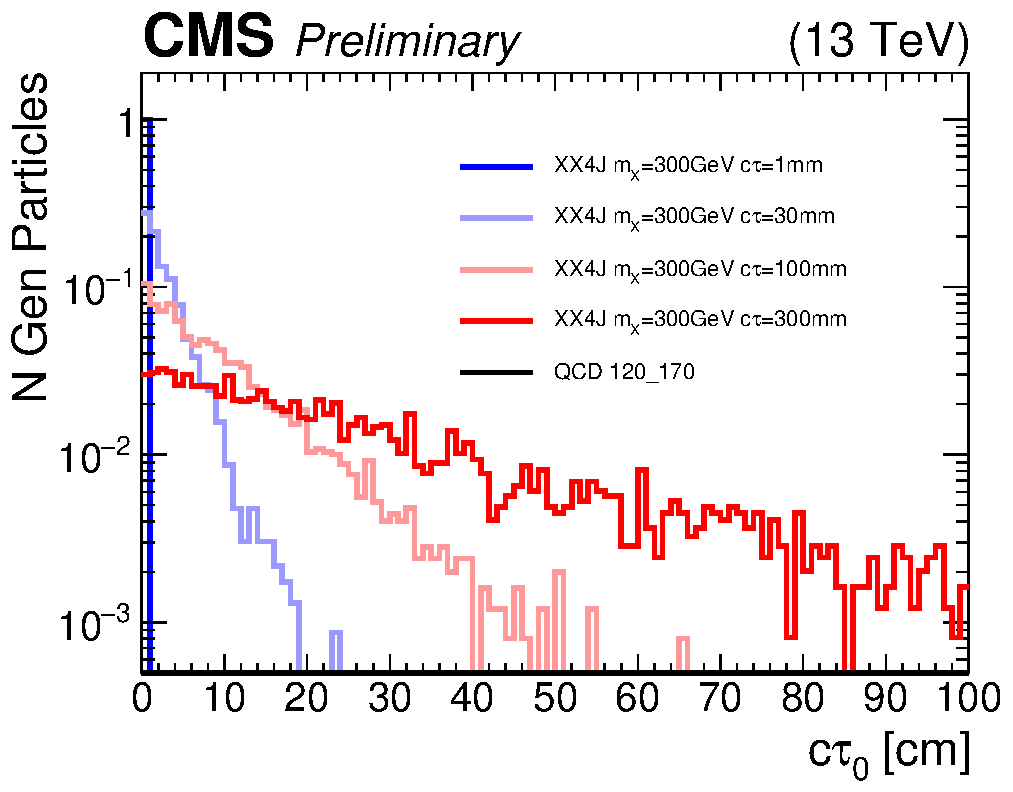
\includegraphics[width=.45\textwidth]{figures/an_jetid/VTX_MATCH_IP/XX4J_ctau0}
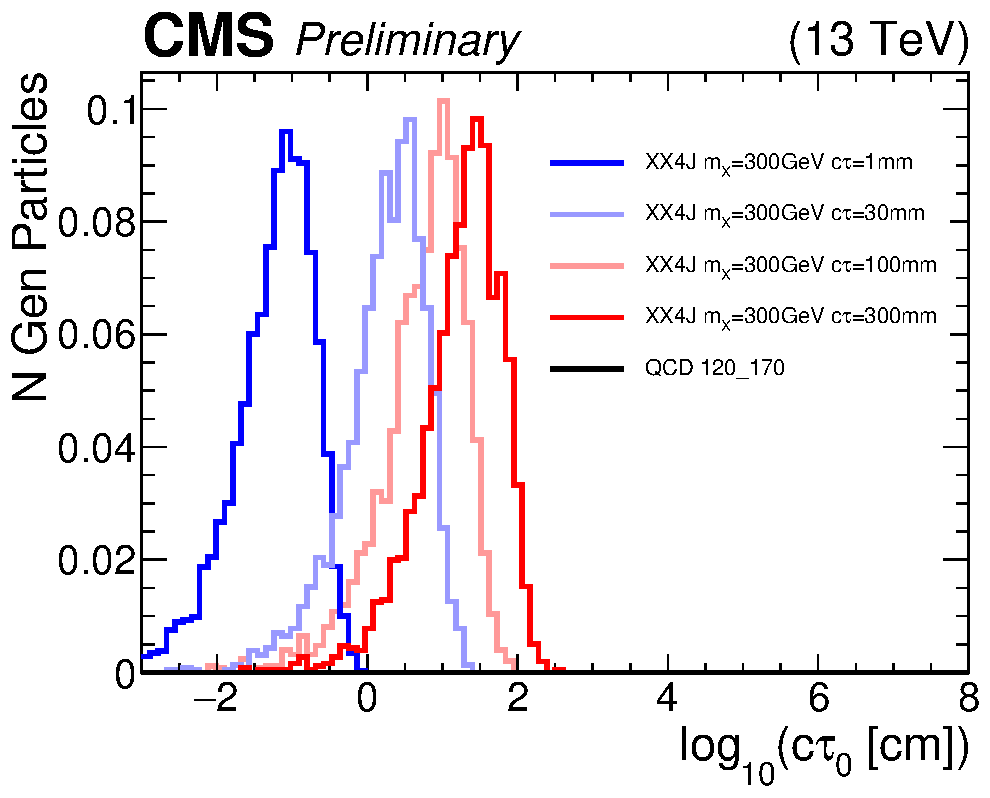
\includegraphics[width=.45\textwidth]{figures/an_jetid/VTX_MATCH_IP/XX4J_log_ctau0}
\end{center}
\caption{The proper lifetime  of the XX4J samples. The samples are generated with exponential lifetime distributions
$e^{- x / c\tau_0}$ which have mean $c\tau_0$ and exponential slope $1/c\tau_0$.}
\label{fig:xx4j_ctau0}
\end{figure}

\begin{figure}
\begin{center}
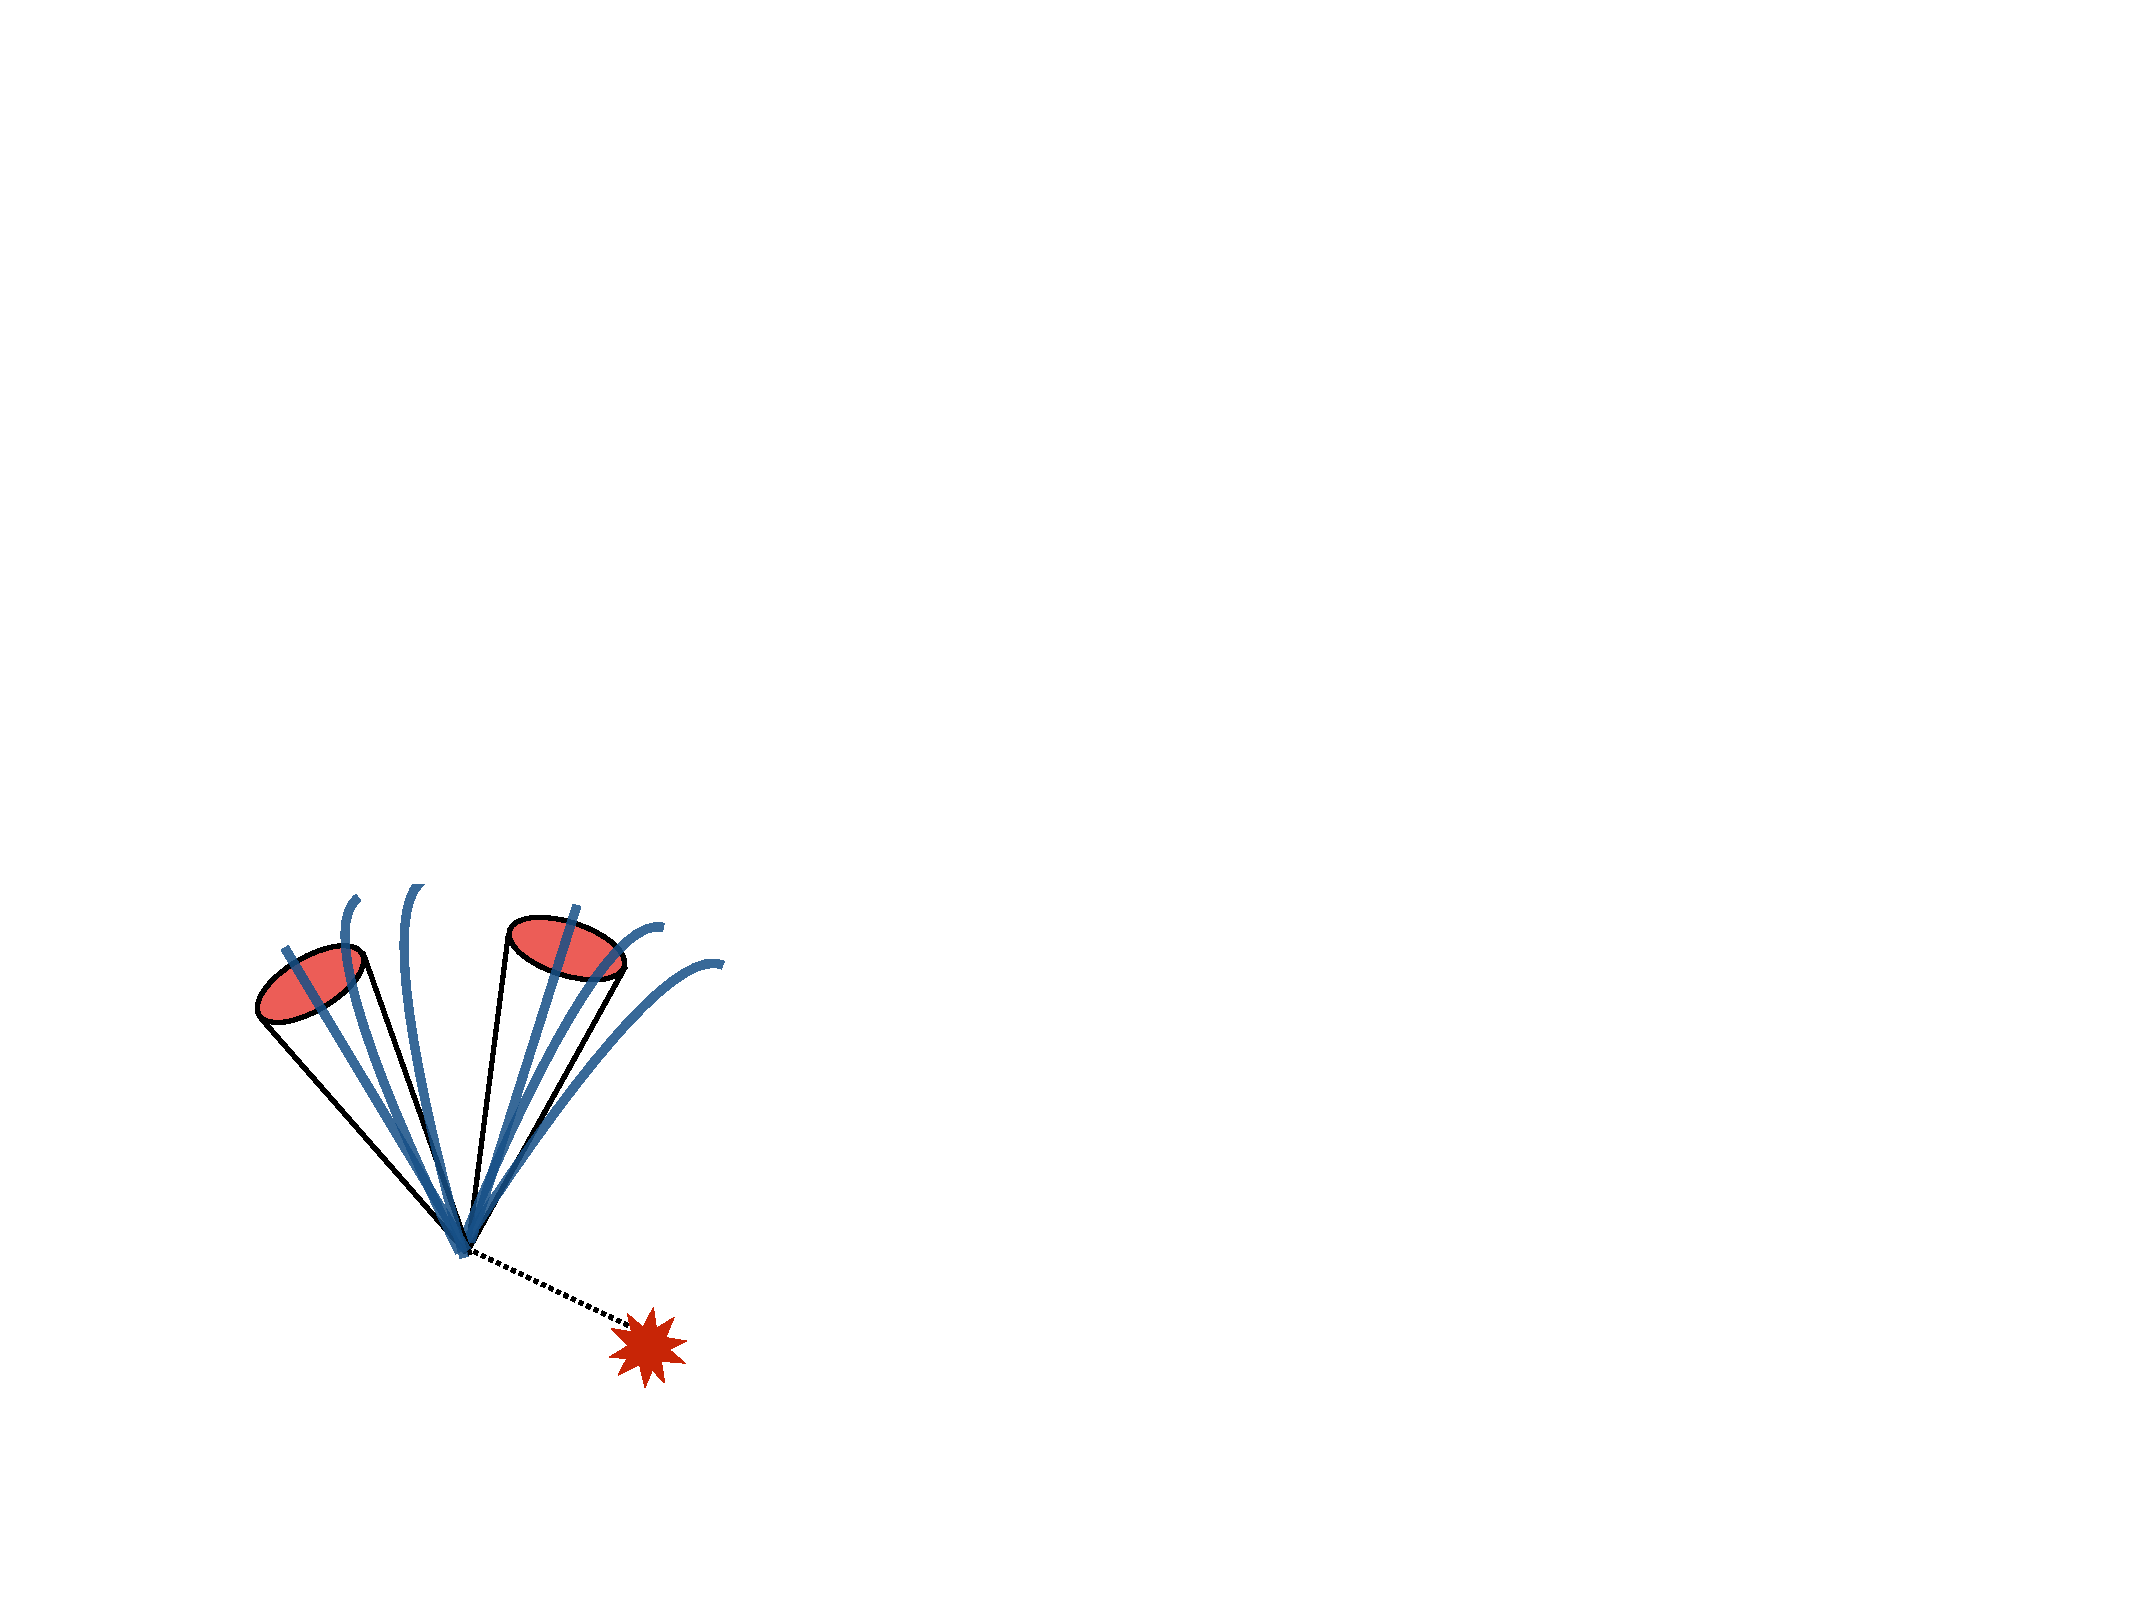
\includegraphics[width=.38\textwidth]{figures/an_jetid/DIAGRAMS/dijet_gun}
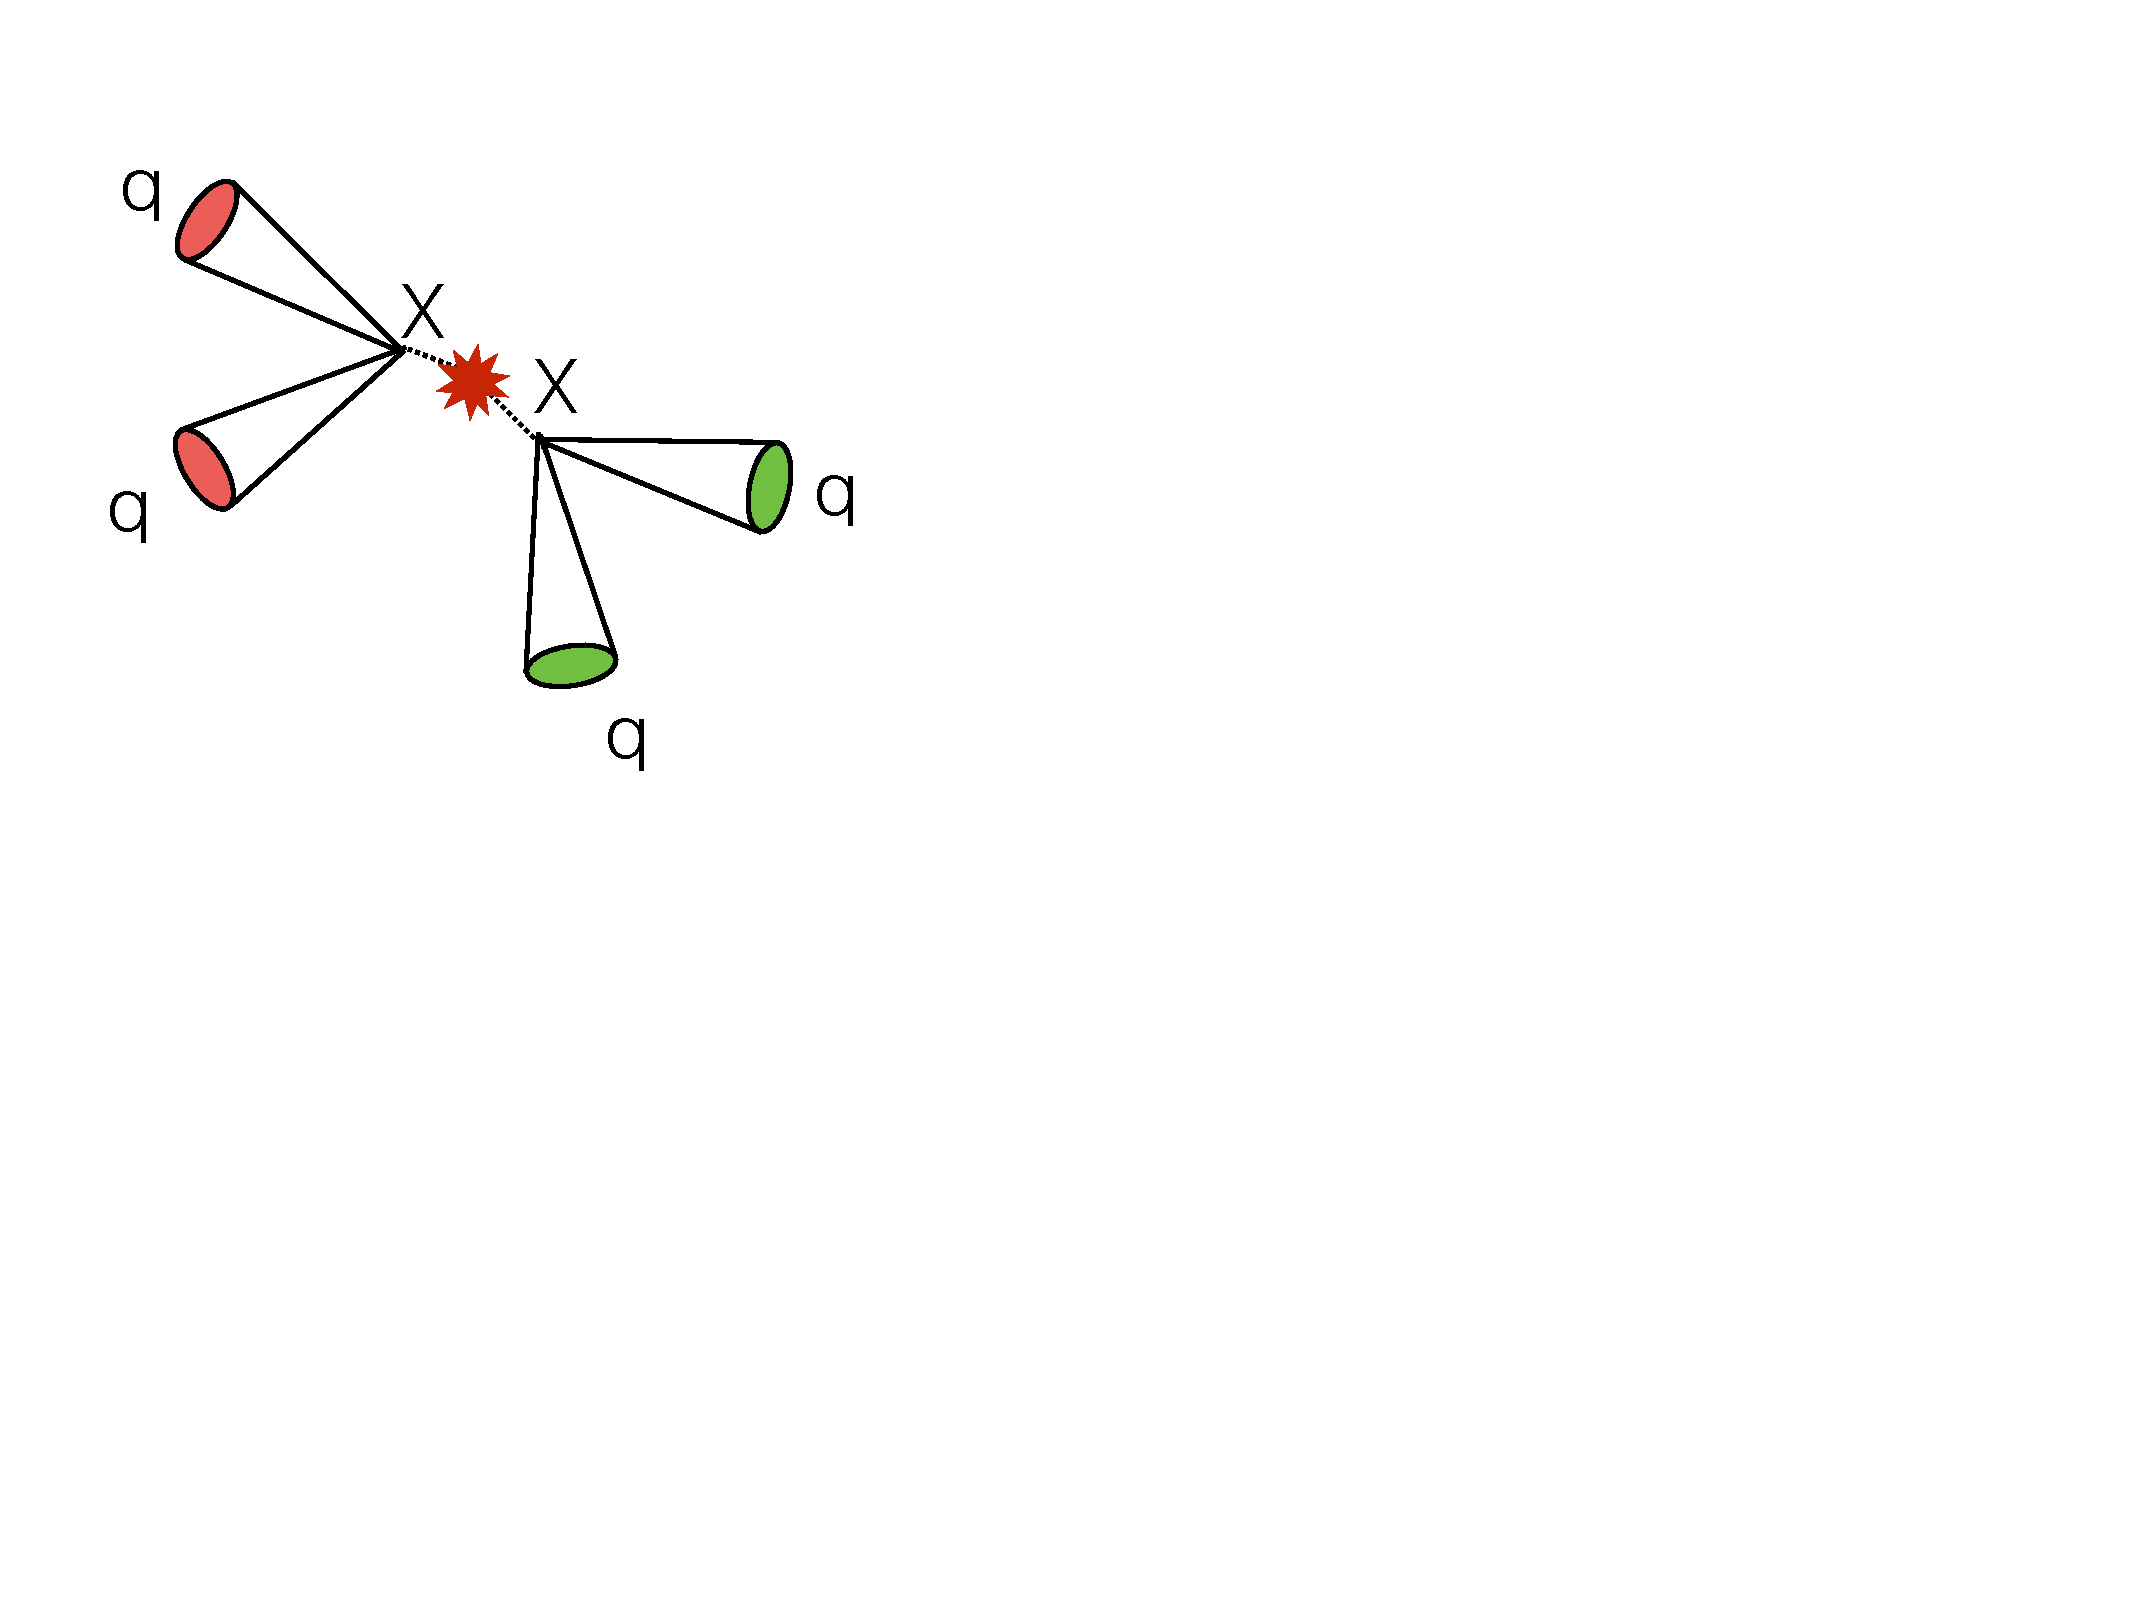
\includegraphics[width=.58\textwidth]{figures/an_jetid/DIAGRAMS/xx4j_diagram}
\end{center}
\caption{The topology of the two samples used in the study GUN (left) and  XX4J (right) }
\label{fig:xx4j_gun}
\end{figure}
Two signal samples are used to study displaced identification which we will refer to as XX4J and GUN. Both samples are generated
using Pythia 8 \cite{Sjostrand:2007gs}. 

The XX4J sample consists of the direct pair production of two neutral $X^{0}$'s with finite lifetime.  
Each $X^{0}$ decays to $u$,$d$,$s$,$c$, and $b$ pairs with equal probability. This
sample is generated with a flat pileup distribution between 10 and 50 interactions
from 25 ns bunch crossings. It is important
to note these samples will contain prompt jets from pile up interactions as 
well as from initial state radiation. 
In this sample, variables for displaced jet identification generally have two distinct populations of jets. The samples are generated
with varied lifetimes and masses (Figure \ref{fig:xx4j_ctau0}). Each $X^0$ has an
exponential lifetime distribution $e^{-x / c\tau_0}$ with mean $c\tau_0$. 
\begin{figure}
\begin{center}
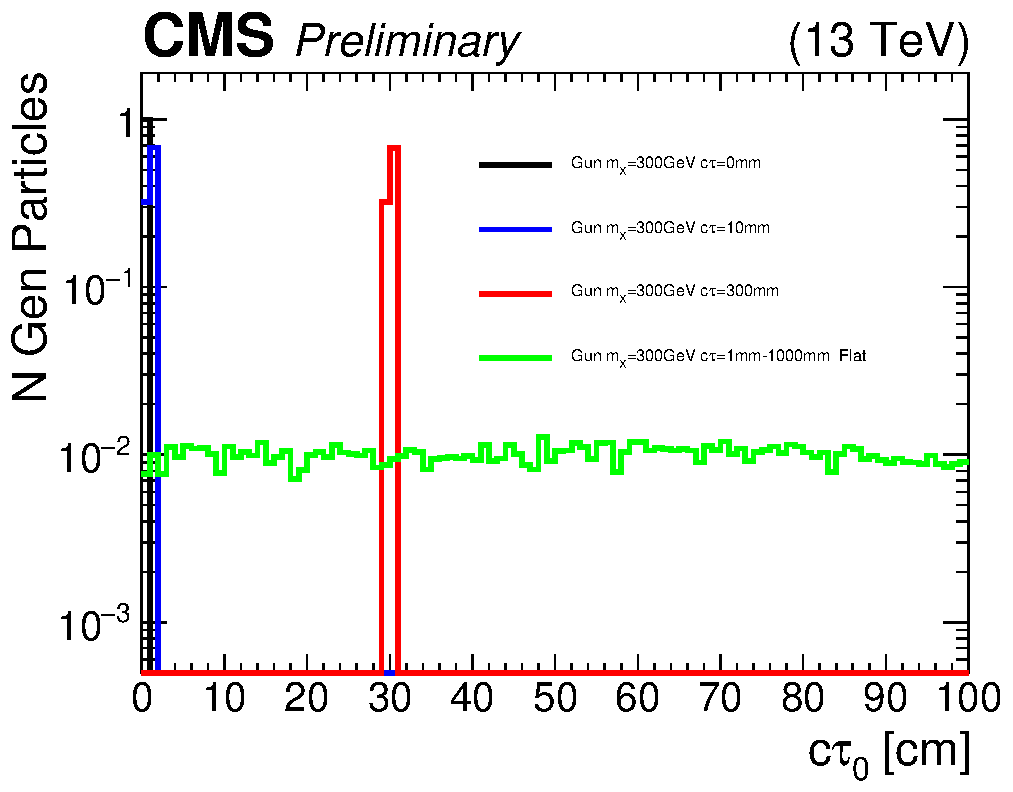
\includegraphics[width=.45 \textwidth]{figures/an_jetid/VTX_MATCH_IP/GUN_ctau0}
\end{center}
\caption{The proper lifetime of the GUN samples. The samples are generated with either flat, or delta function
$\delta(c\tau_0 - c\tau_0')$ lifetime distributions}
\label{fig:gun_ctau0}
\end{figure}

The GUN sample is a single long-lived particle gun. 
This sample is generated by producing a single $X^0$ particle with flat kinematic distributions $50 < p_{\textrm{t}} < 500$~GeV and 
flat $-2.4< \eta < 2.4$. The $X^{0}$ decays to a pair of $d$ quarks with 100\% branching fraction
(or b quarks with 100\% fraction when noted). The resonance is decayed within Pythia and passed directly to
showering and hadronization bypassing all process level Pythia effects: initial
state radiation, final state radiation, and beam remnants. Furthermore, the event is reconstructed without pileup mixing. This sample
is generated to have a sample of reconstructed tracks that originate from a displaced vertex without the complications of correctly associating
the displaced tracks to calorimeter deposits. One important side effect of simulating without pileup is the lack of a reconstructed primary vertex. 
As the only vertex in the event is far from the luminous region of the beam, the primary vertex fitting fails to produce a vertex.

The proper lifetime distribution of the sample is chosen to be either a delta function $\delta(c\tau_0 - c\tau_0')$ or 
flat between 1mm and 1000mm (Figure \ref{fig:gun_ctau0}). Additionally two prompt GUN samples are built for comparison.
One sample with a proper lifetime of 0 mm decaying to two b-quarks and one sample with lifetime 0mm decaying to two d-quarks. The decay length 
in the lab frame will differ by a factor $\gamma\beta$ from the proper lifetime. 
%% All generator level process effects
%% have been turned off including artifacts of the beam remnants, initial state radiation, and final state radiation.
%% Each event will thus contain a single displaced vertex and no contamination from real prompt tracks. 
%% The only prompt tracks in the event are due to mis-reconstruction. 

%% \begin{verbatim}
%%     PGunParameters = cms.PSet(
%%         ParticleID = cms.vint32(35),
%%         AddAntiParticle = cms.bool(False),
%%         MinPhi = cms.double(-3.14159265359),
%%         MaxPhi = cms.double(3.14159265359),
%%         MinPt = cms.double(50.0),
%%         MaxPt = cms.double(500.0),
%%         MinEta = cms.double(-2.4),
%%         MaxEta = cms.double(2.4)
%%         ),}
%% \end{verbatim}

%% \begin{figure}
%% \begin{center}
%% 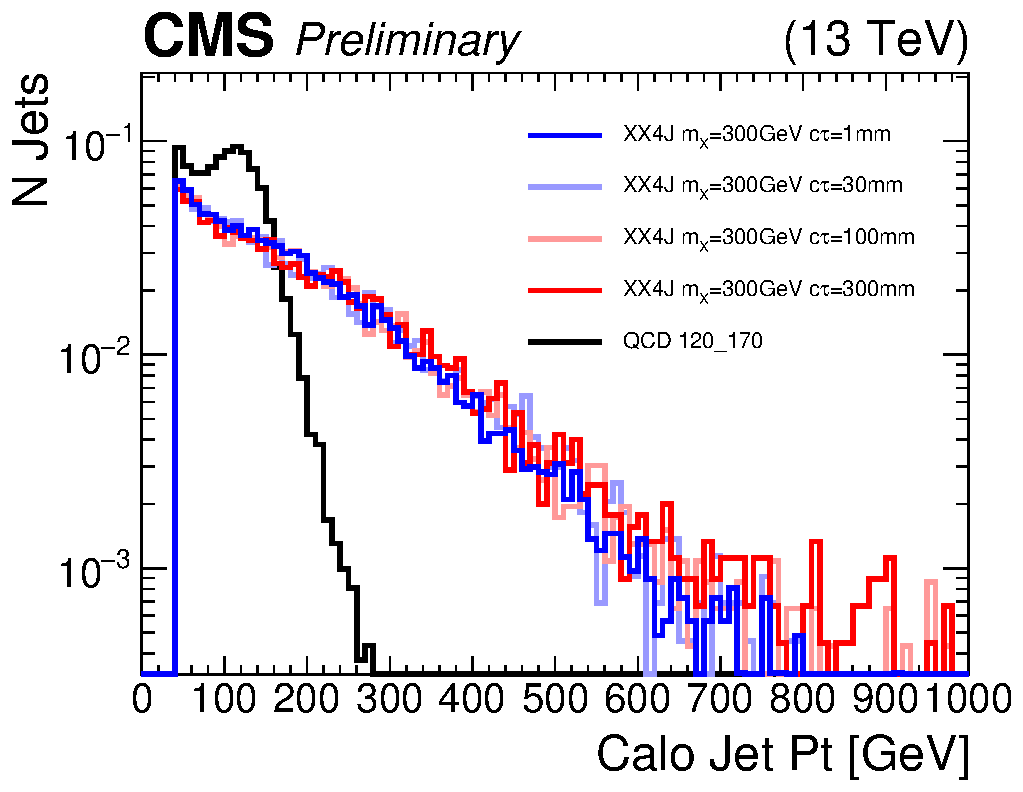
\includegraphics[width=.45\textwidth]{figures/an_jetid/VTX_MATCH_IP/XX4J_caloJetPt}
%% 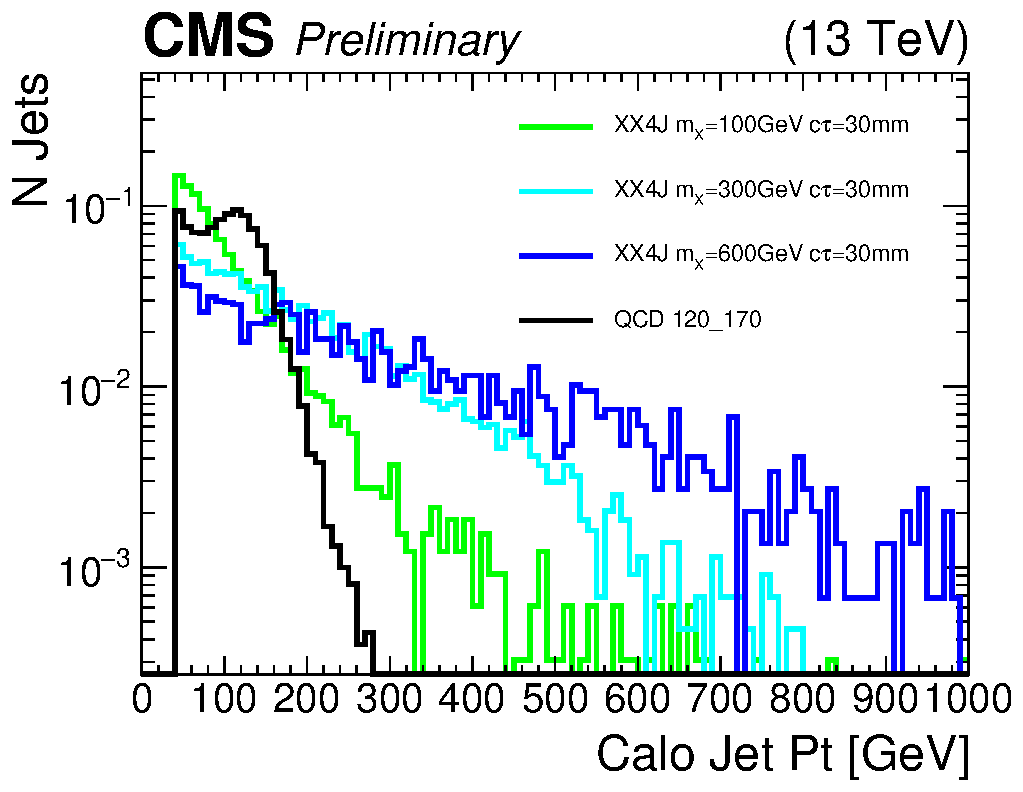
\includegraphics[width=.45\textwidth]{figures/an_jetid/VTX_MATCH_IP/XX4J_MASS_caloJetPt}
%% 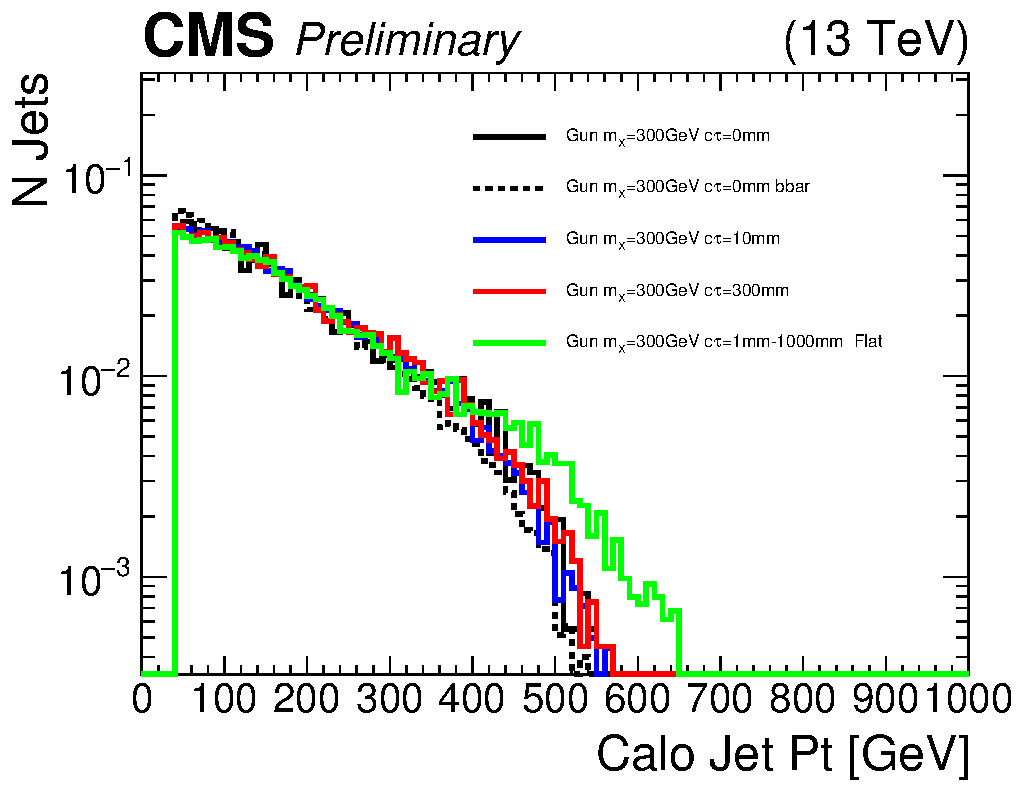
\includegraphics[width=.45\textwidth]{figures/an_jetid/VTX_MATCH_IP/GUN_caloJetPt}
%% \end{center}
%% \caption{The calo jet $p_{t}$ of the \textbf{XX4J} and $GUN$ samples.}
%% \label{fig:xx4j_gun_caloJetPT}
%% \end{figure}

%% The reconstructed calo jet transverse momentum for varied lifetimes is not especially sensitive to the lifetime of the decaying $X^0$ (Fig. \ref{fig:xx4j_gun_caloJetPT})
%% until very long lifetimes. The flat lifetime gun sample develops high transverse momentum (relative to the shorter lifetime) jets when the long lived $X^0$ decays at 
%% a transverse distance far enough from the beam line to be reconstructed as a single jet, or
%% decaying entirely inside the calorimeter. 


\section{Displaced Jet Tagging Variables}


\subsection{Impact Parameter Information}

%% \begin{figure}
%% \begin{center}
%% 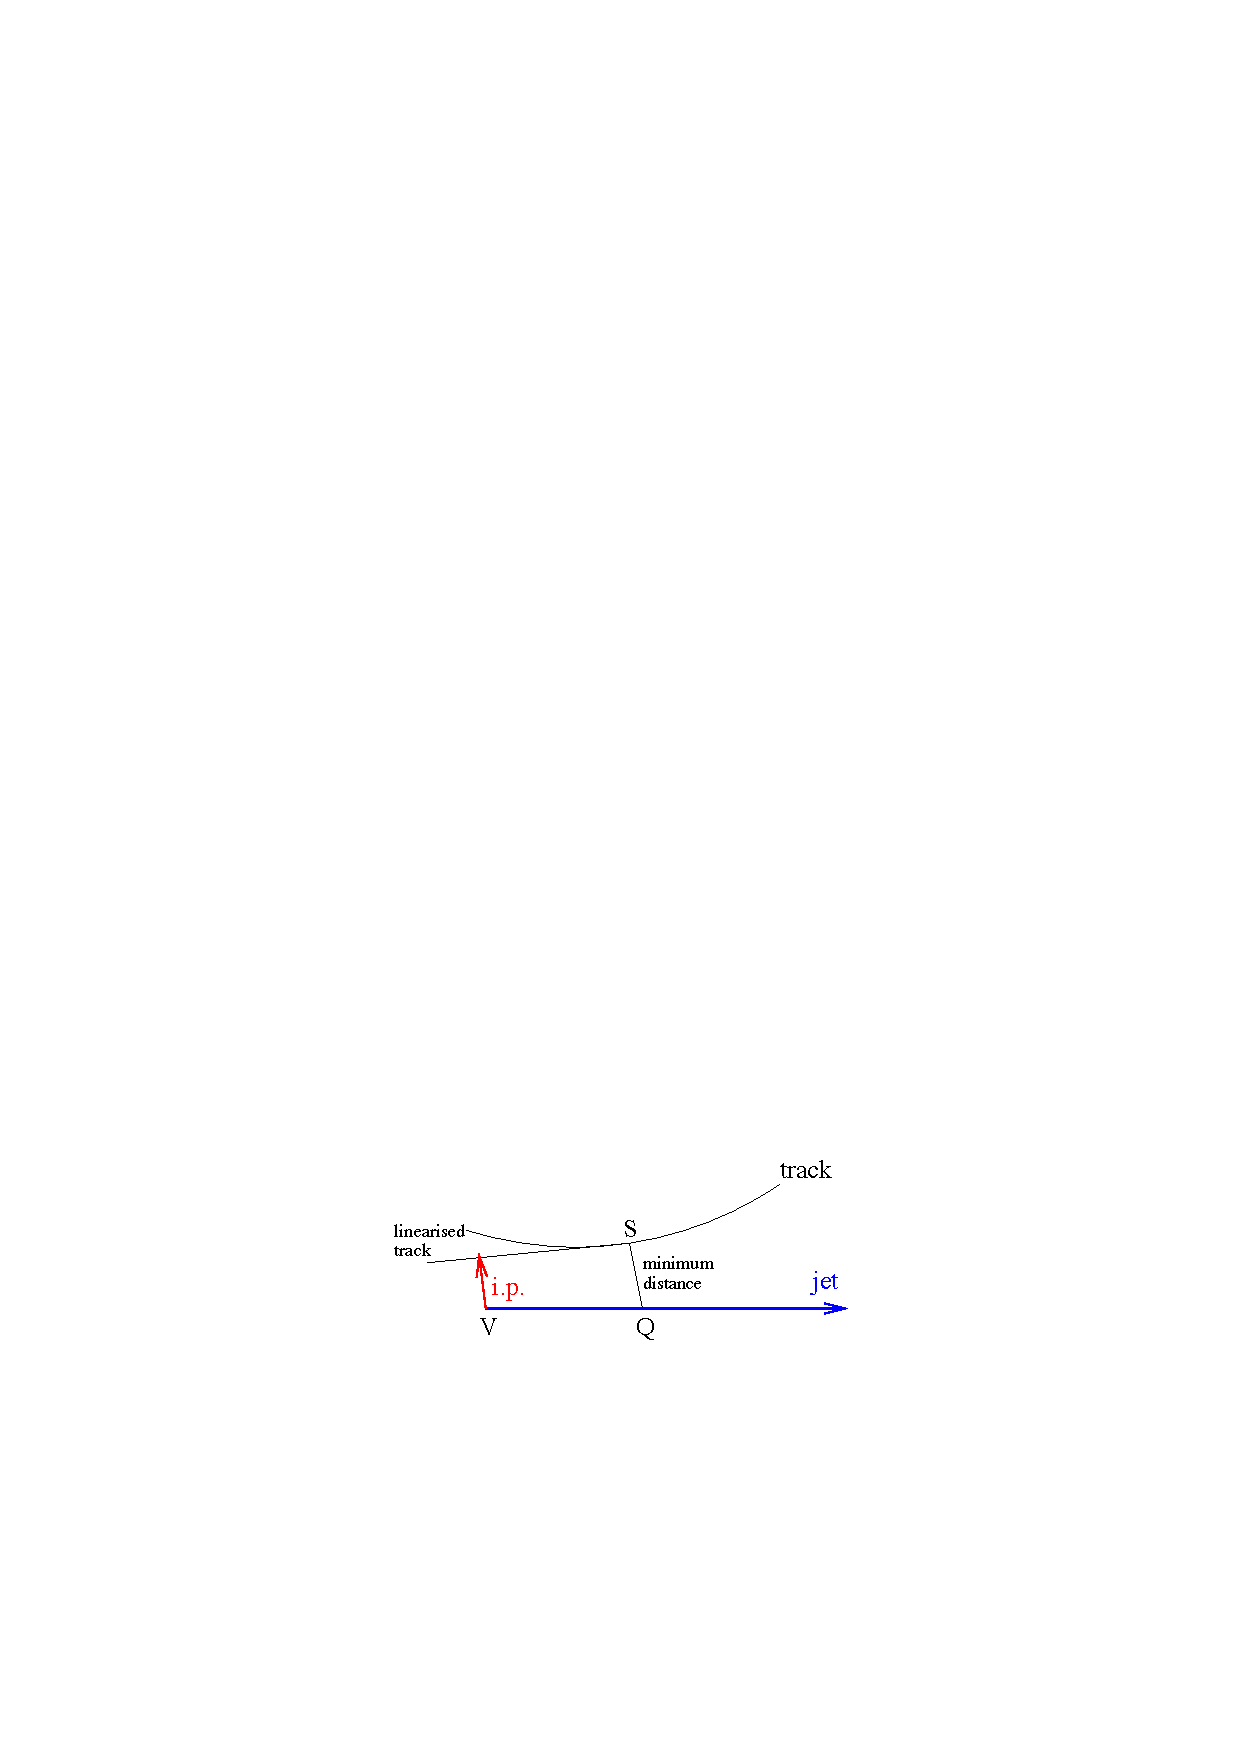
\includegraphics[width=.7\textwidth]{figures/an_jetid/DIAGRAMS/ip_diagram}
%% \end{center}
%% \caption{Diagram depicting the impact parameter calculation. $V$ is the position of the primary vertex. $\vec j = \vec{VQ}$ is the direction of the calo jet. $S$ is the point on the track extrapolation backward from the inner hit which is closest to the jet axis. From $S$ the track is
%% linearized and extrapolated backwards. The impact parameter magnitude is the minimal distance on the linearized track from the primary vertex. We
%% will denote the vector from the primary vertex to the point of minimal distance on the linearized track as $\vec{IP}$}
%% \label{fig:ipdiagram}
%% \end{figure}

%% \begin{figure}
%% \begin{center}
%% 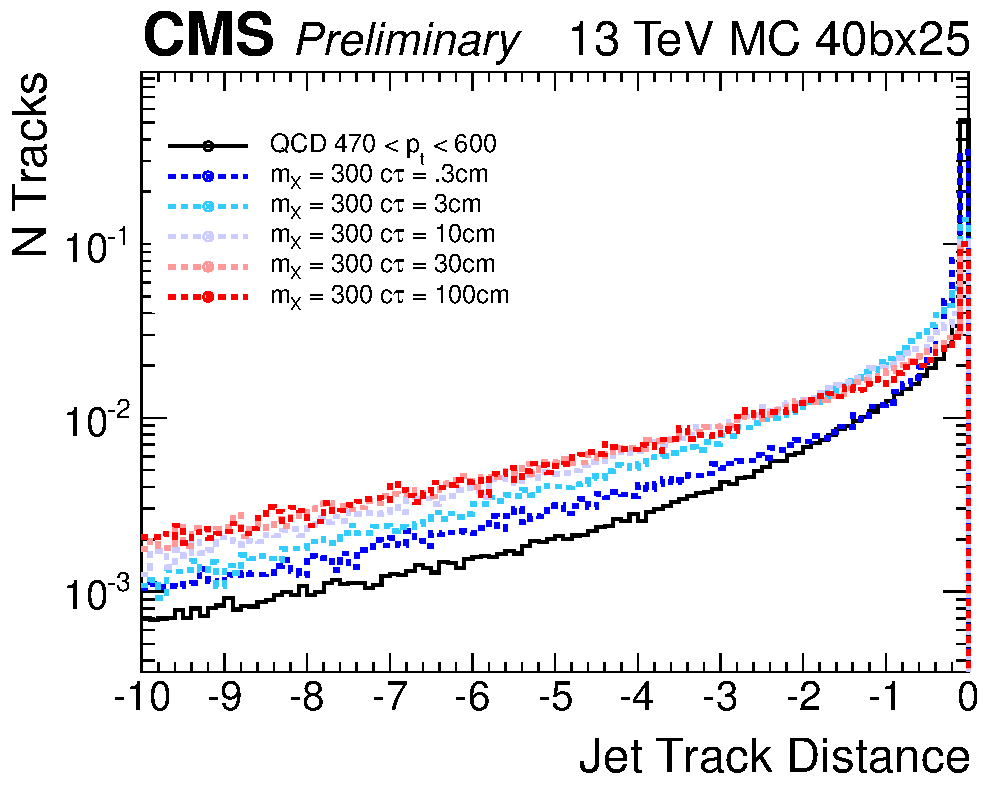
\includegraphics[width=.7\textwidth]{figures/an_jetid/VTX_MATCH_IP/liTrackDistanceJetAxis}
%% \end{center}
%% \caption{The closest distance between the jet axis and track}
%% \label{fig:distance}
%% \end{figure}
The tracks originating from a decay at a displaced vertex will have large impact parameters relative
to the true primary vertex. The impact parameter is calculated by starting from the particle trajectory at the
innermost measurement point  and extrapolating backward in the helix. The minimum distance from the extrapolated
track to the primary vertex gives the magnitude of the impact parameter. The vector pointing from the primary vertex to the point of 
minimum distance is $\vec{IP}$. The distance between the jet axis and the closest position on the track helix was also investigated
 (Figure \ref{fig:jetDist}), but was found to be less effective at separating the signal and background. 

Impact parameter significance $IP_{\textrm{sig}}$ is introduced to the account of the tracking resolution. The significance is the impact parameter divided by the error
on the measurement. For decays within $10$~mm using $IP_{\textrm{sig}}^{\textrm{2D}}$ gives improvements in signal background separation relative to the absolute impact parameter value Figure \ref{fig:ip_vs_ipsig}.
\begin{figure}
\begin{center}
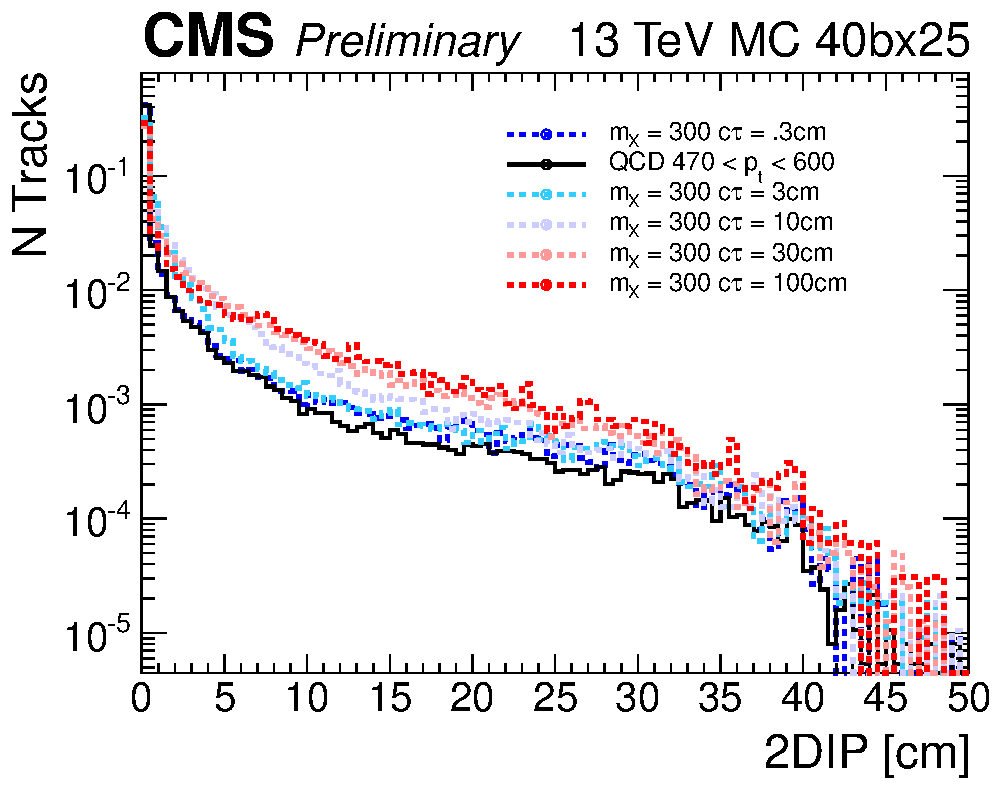
\includegraphics[width=.45\textwidth]{figures/an_jetid/VTX_MATCH_IP/liTrackIP2D}
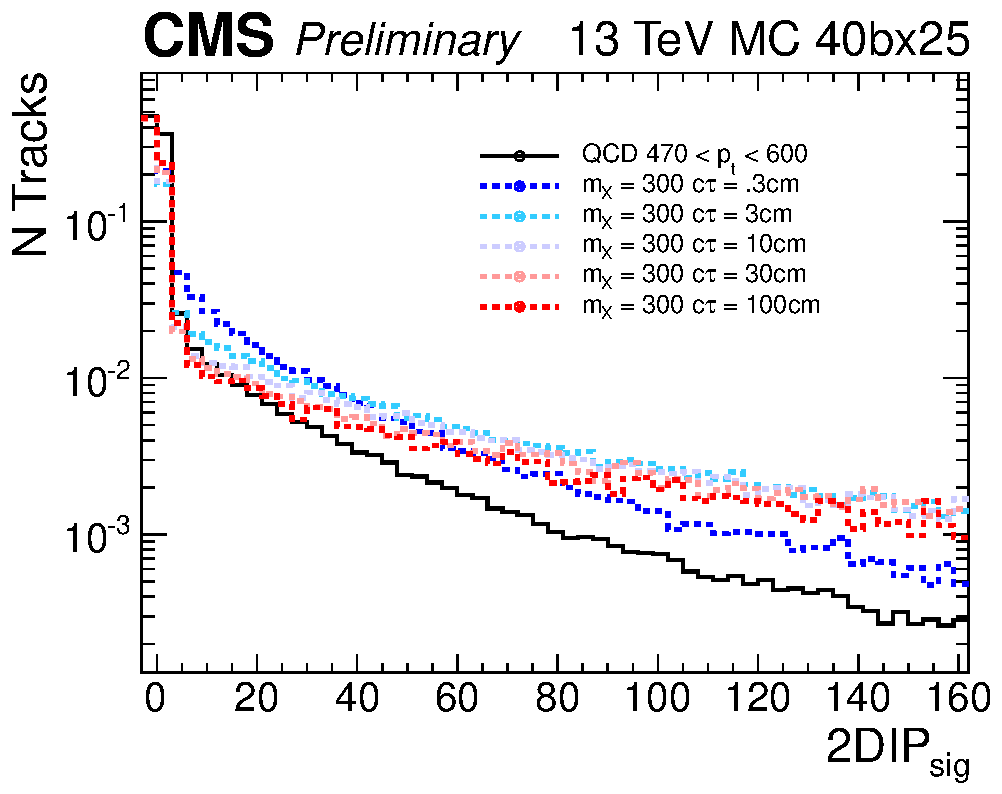
\includegraphics[width=.45\textwidth]{figures/an_jetid/VTX_MATCH_IP/liTrackIPSig2D}\\
\end{center}
\caption{(left) The 2D impact parameter of tracks matched to calo jets matched to generator quarks with $\Delta R < 0.5$.
 (right) 2D impact parameter significance of the same tracks. All distributions are normalized to 1.}
\label{fig:iptrack}
\end{figure}

\begin{figure}
\begin{center}
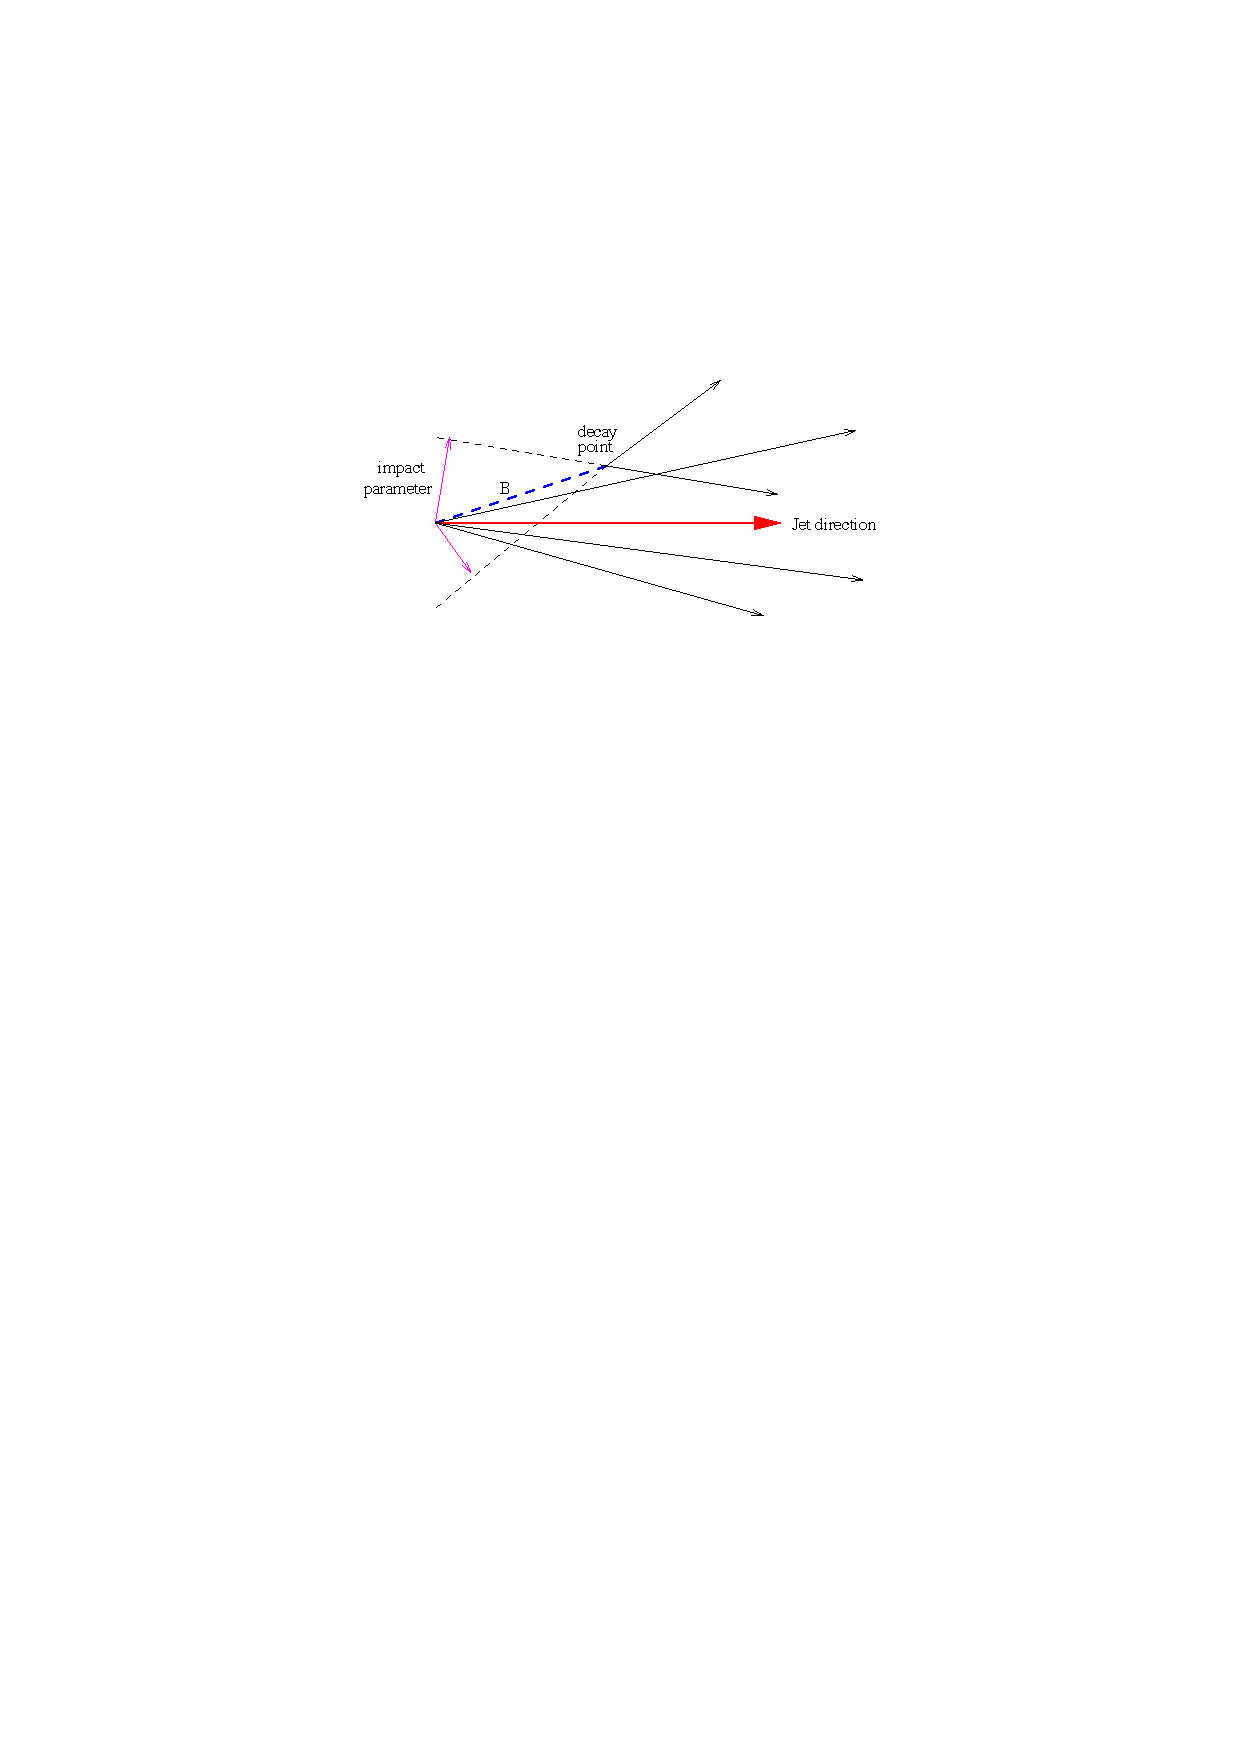
\includegraphics[width=.7\textwidth]{figures/an_jetid/DIAGRAMS/b_diagram}
\end{center}
\caption{Diagram of a B hadron decay showing the mis-alignment of the jet direction and the decay vertex.}
\label{fig:bdiagram}
\end{figure}

\begin{figure}
\begin{center}
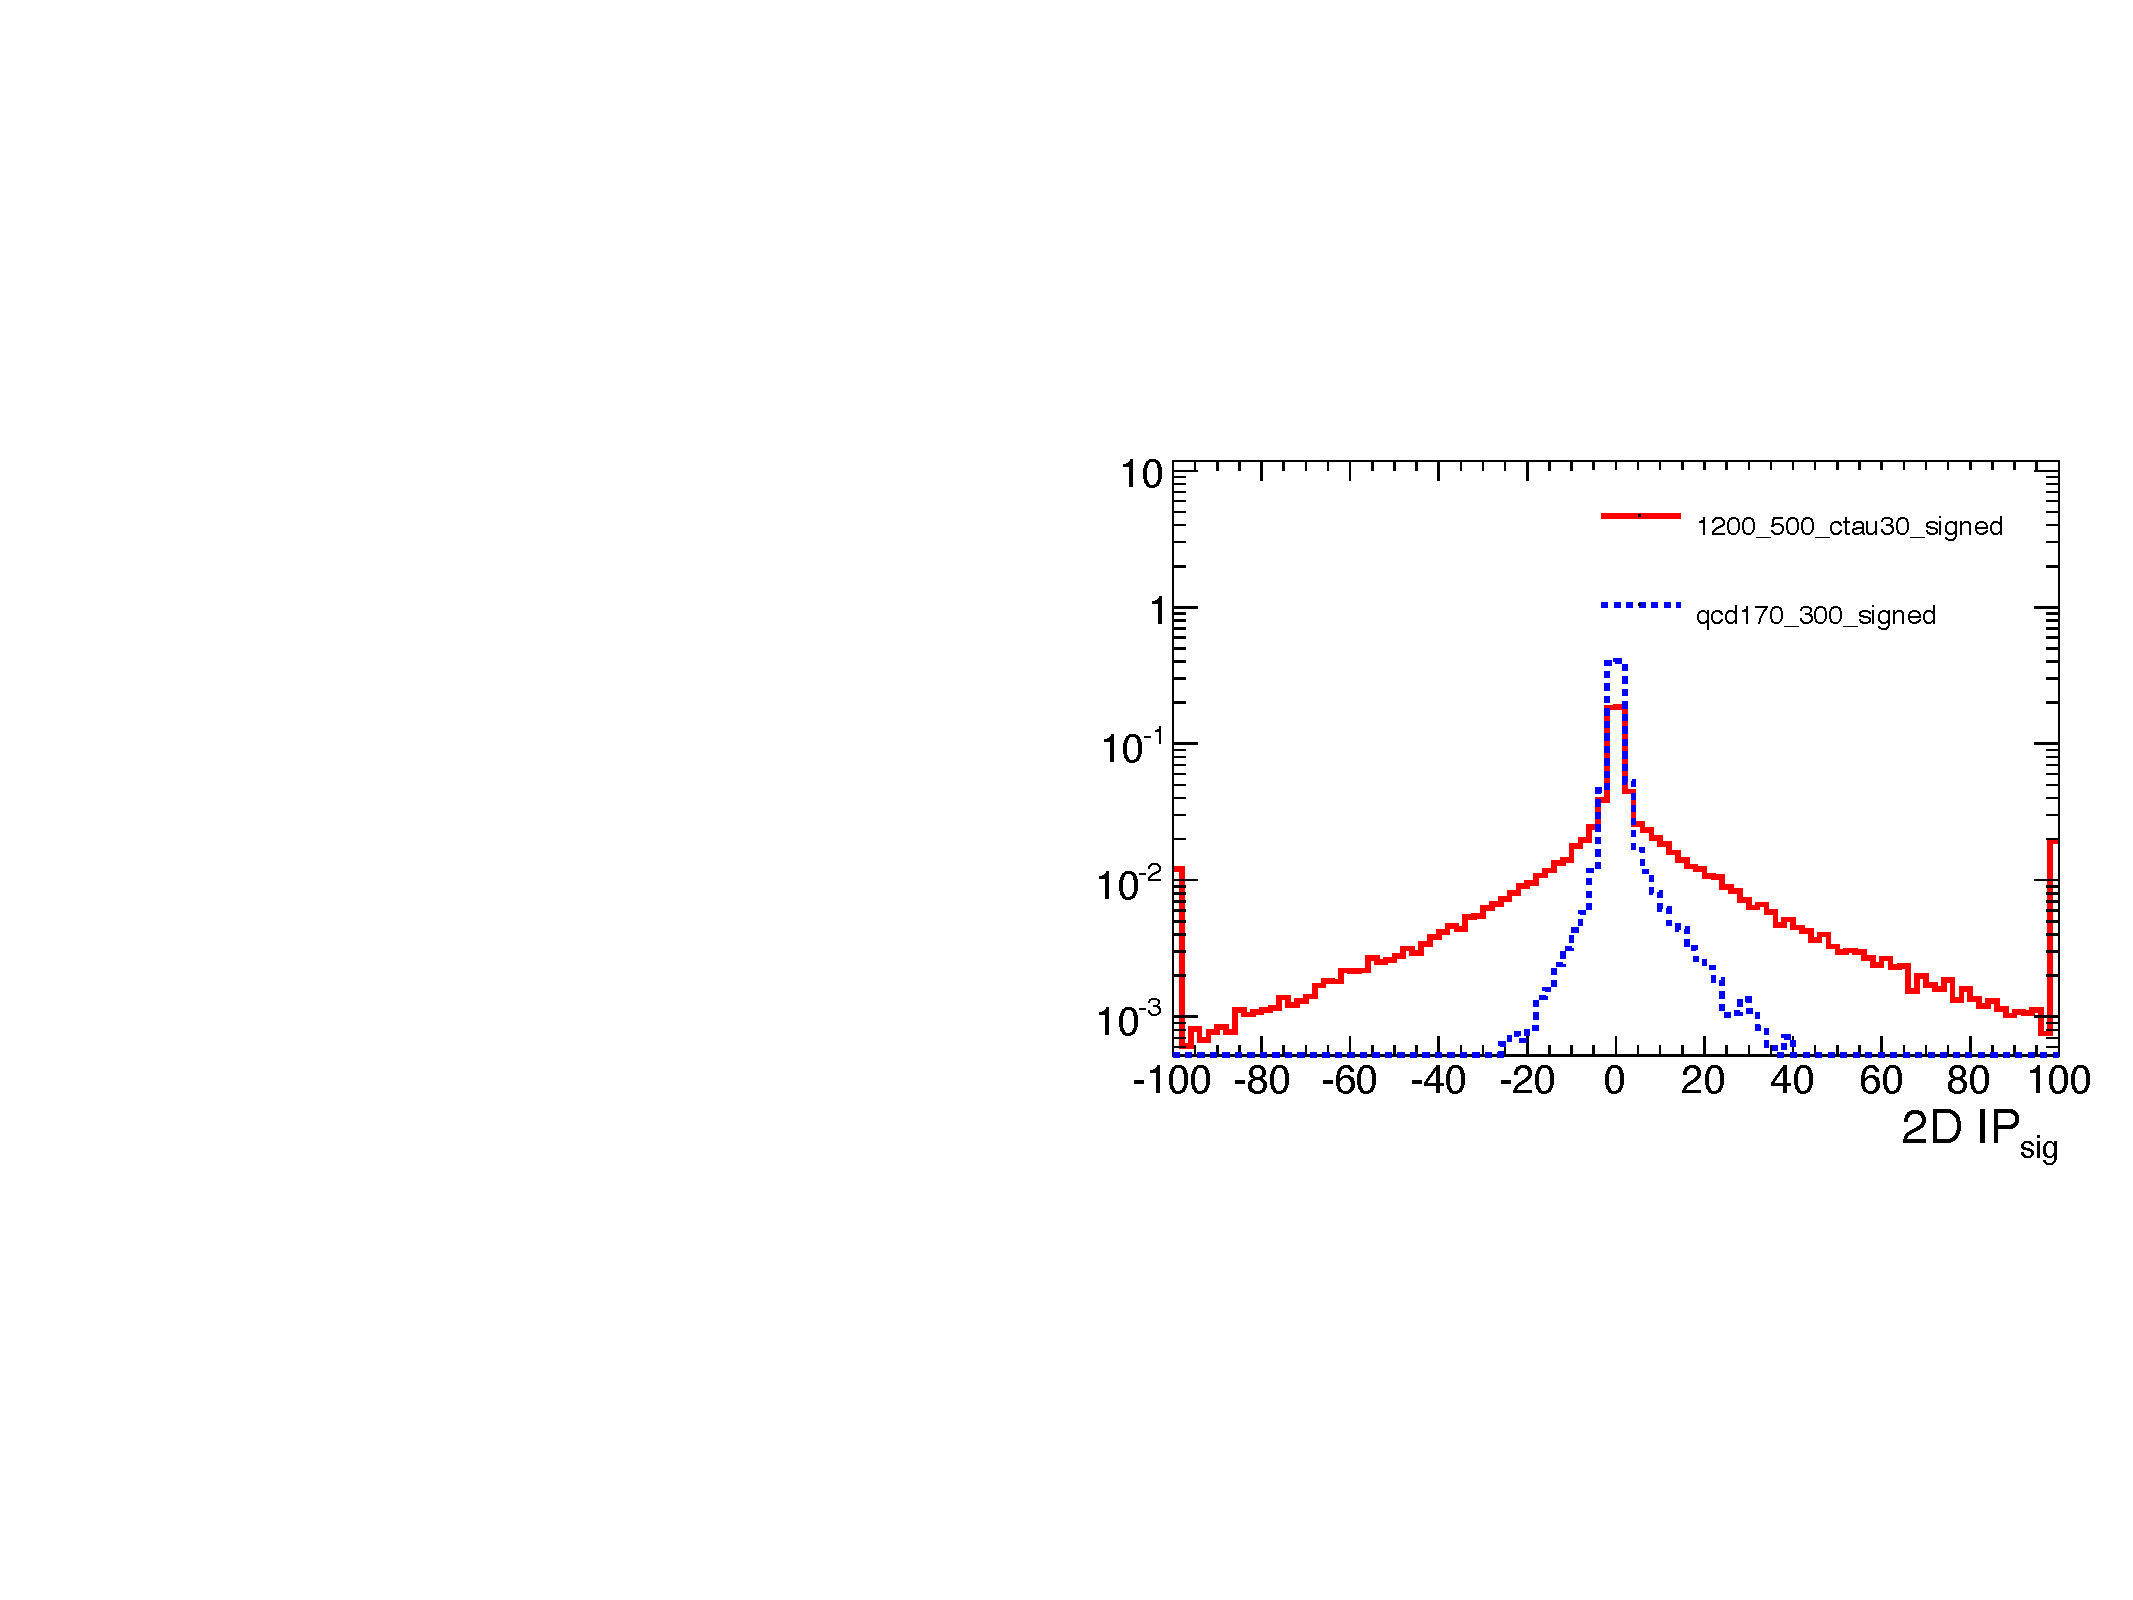
\includegraphics[width=.7\textwidth]{figures/an_jetid/signed_2dipsig}
\end{center}
\caption{The comparison between the $IP_{\textrm{sig}}^{\textrm{2D}}$ of tracks within (i) QCD jets and (ii) the decay of a
 heavy Higgs $H^0=1200$ GeV decaying to two long lived
$X^{0}$ with $m_{X^0}=500$ GeV. The contribution of B mesons producing tracks 
with large positive $IP_{\textrm{sig}}^{\textrm{2D}}$ explains the asymmetry of the QCD distribution.}
\label{fig:2dipsig_sign}
\end{figure}
The sign of the impact parameter is given as the sign of the scalar product between $\vec{IP}$ and  the direction of the jet: $\vec{IP} \cdot \vec j$. 
For B meson decays, the impact parameter of displaced tracks will have positive sign, corresponding to the decay occurring down stream of the jet direction. In simulation is found that heavy long-lived
decays will have large negative IP significance (Figure \ref{fig:2dipsig_sign}). 
Accordingly, the analysis opts to use un-signed IP significance to 
identify displaced jets. Restricting to only positive
impact parameters, as is the standard in $b$-tagging, topologically restricts
 the analysis. Rather, the un-signed significance extends inclusivity. 

It is important to note that as most GUN samples, excluding the prompt samples, do not  have a reconstructed primary vertex, a fake primary vertex with a nominal error is introduced in the calculation. This biases the impact parameter significance relative to the XX4J.
\begin{figure}
\begin{center}
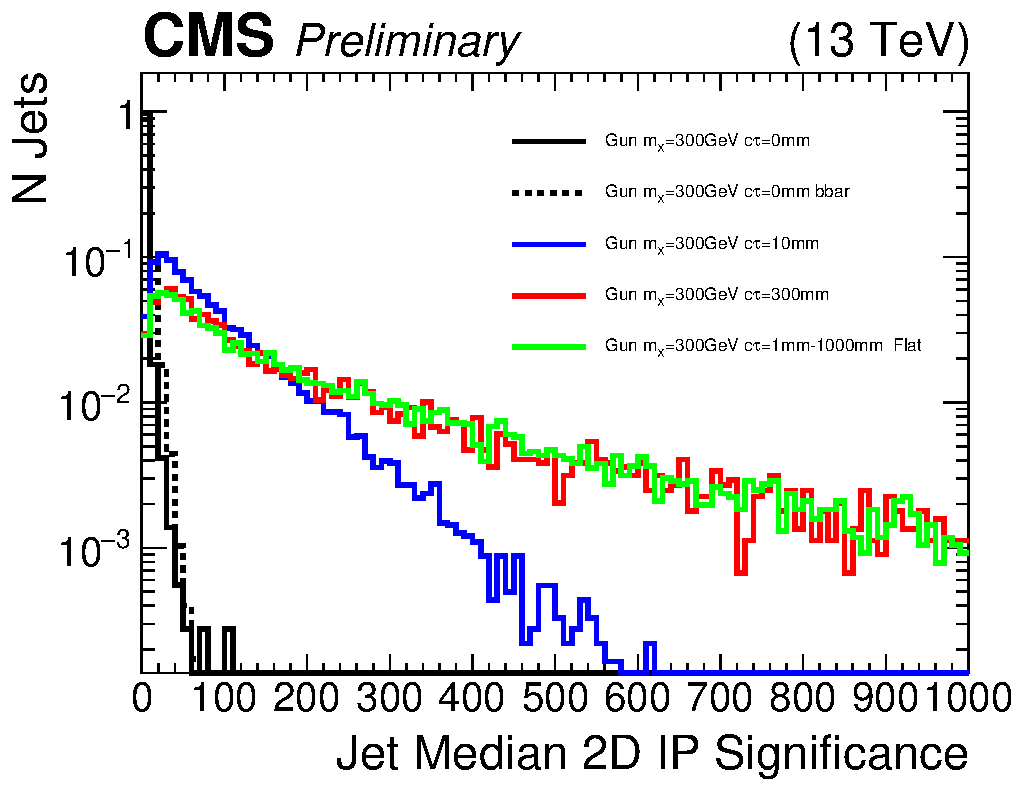
\includegraphics[width=.45\textwidth]{figures/an_jetid/VTX_MATCH_IP/GUN_jetMedianIPSig2D}
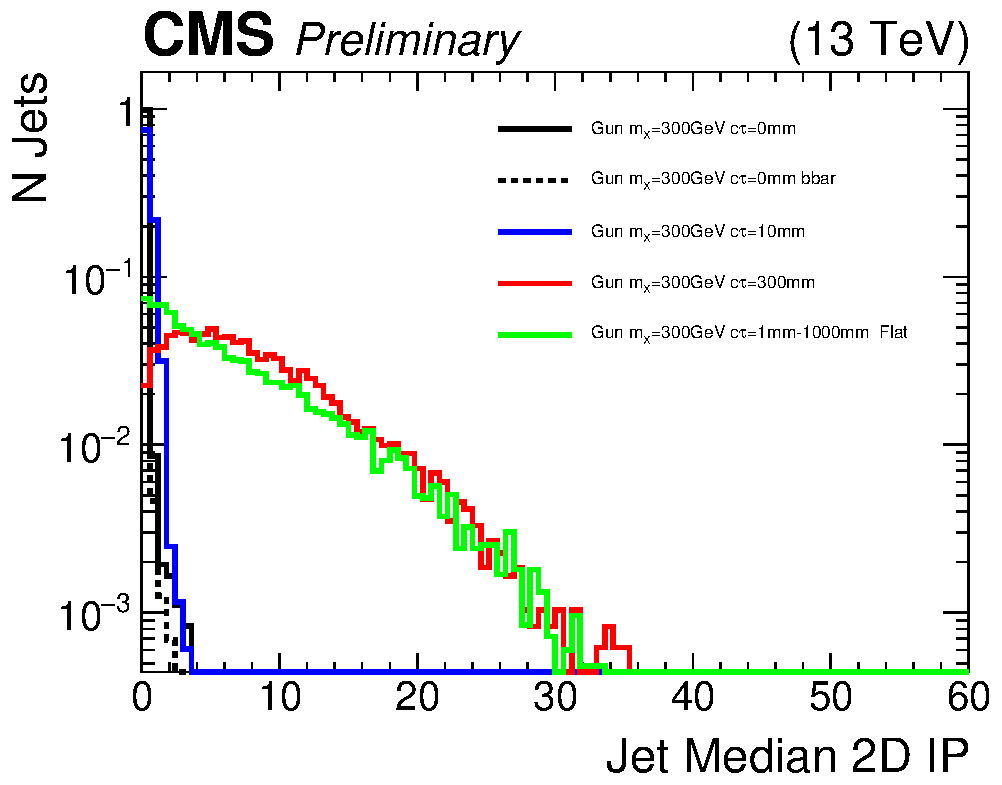
\includegraphics[width=.45\textwidth]{figures/an_jetid/VTX_MATCH_IP/GUN_jetMedianIP2D}
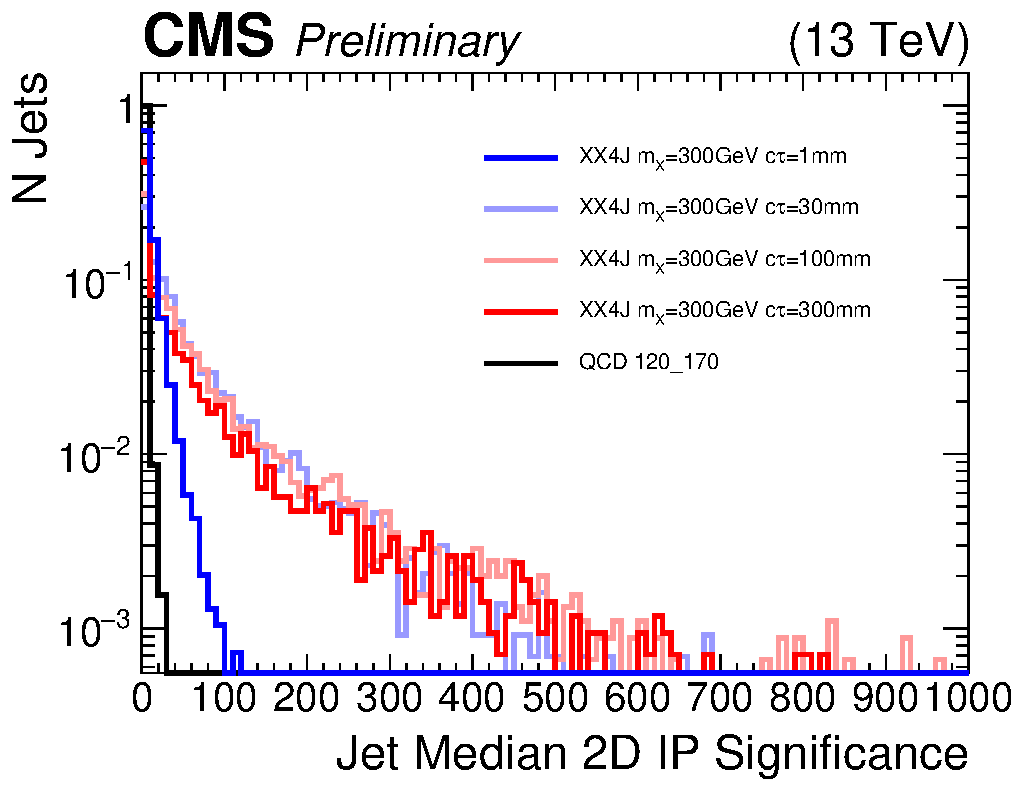
\includegraphics[width=.45\textwidth]{figures/an_jetid/VTX_MATCH_IP/XX4J_jetMedianIPSig2D}
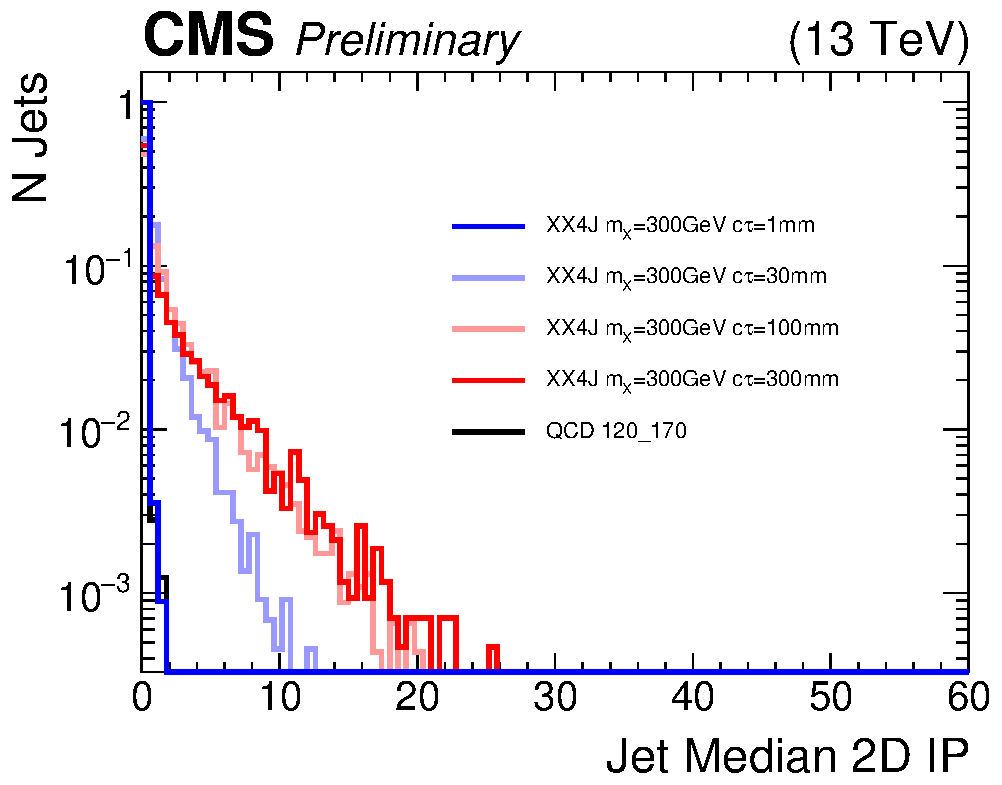
\includegraphics[width=.45\textwidth]{figures/an_jetid/VTX_MATCH_IP/XX4J_jetMedianIP2D}
\end{center}
\caption{Unsigned 2D impact parameter for the XX4J and GUN samples}
\label{fig:ip_vs_ipsig}
\end{figure}

\begin{figure}
\begin{center}
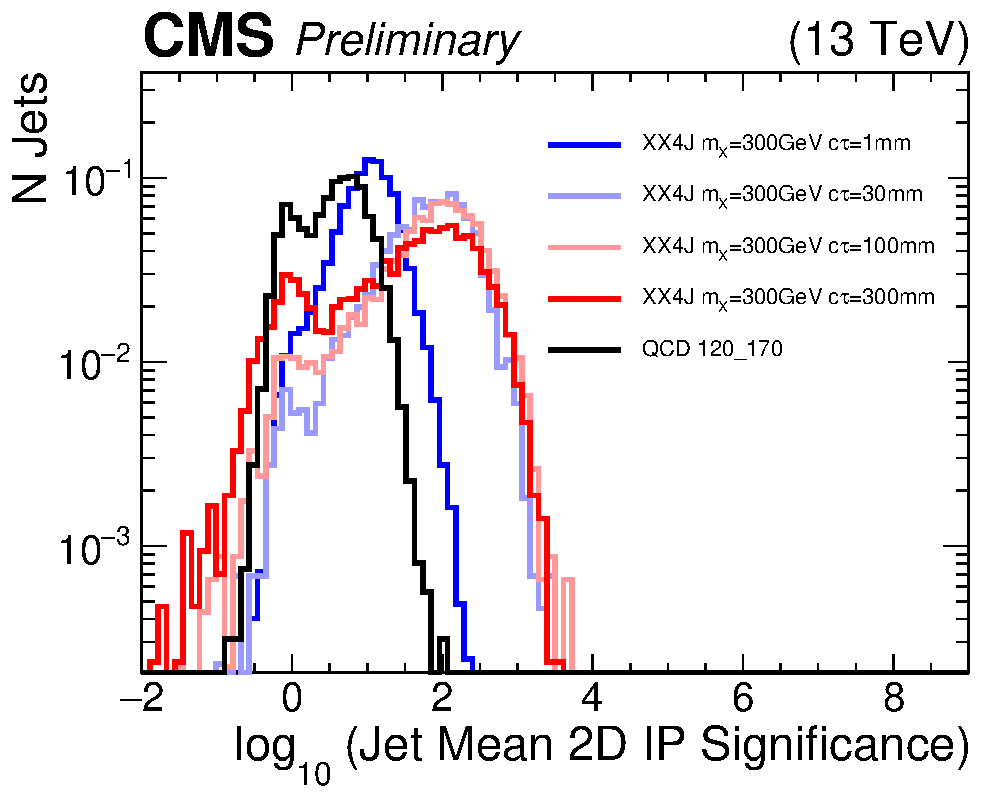
\includegraphics[width=.45\textwidth]{figures/an_jetid/VTX_MATCH_IP/XX4J_log_jetMeanIPSig2D}
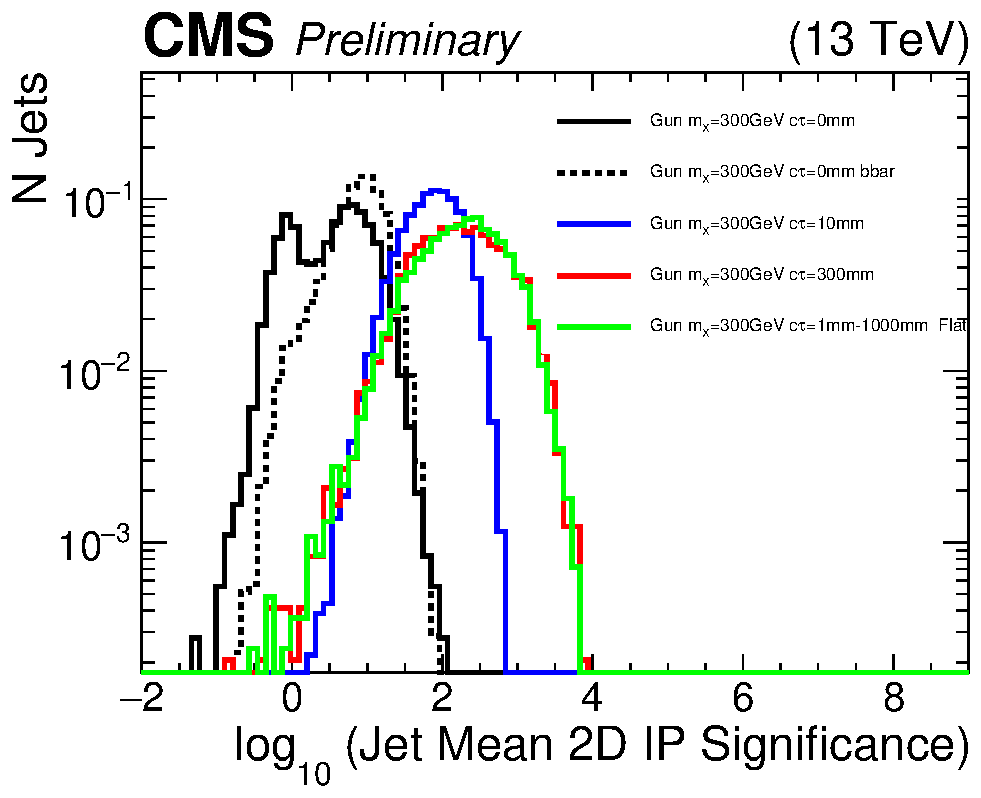
\includegraphics[width=.45\textwidth]{figures/an_jetid/VTX_MATCH_IP/GUN_log_jetMeanIPSig2D}
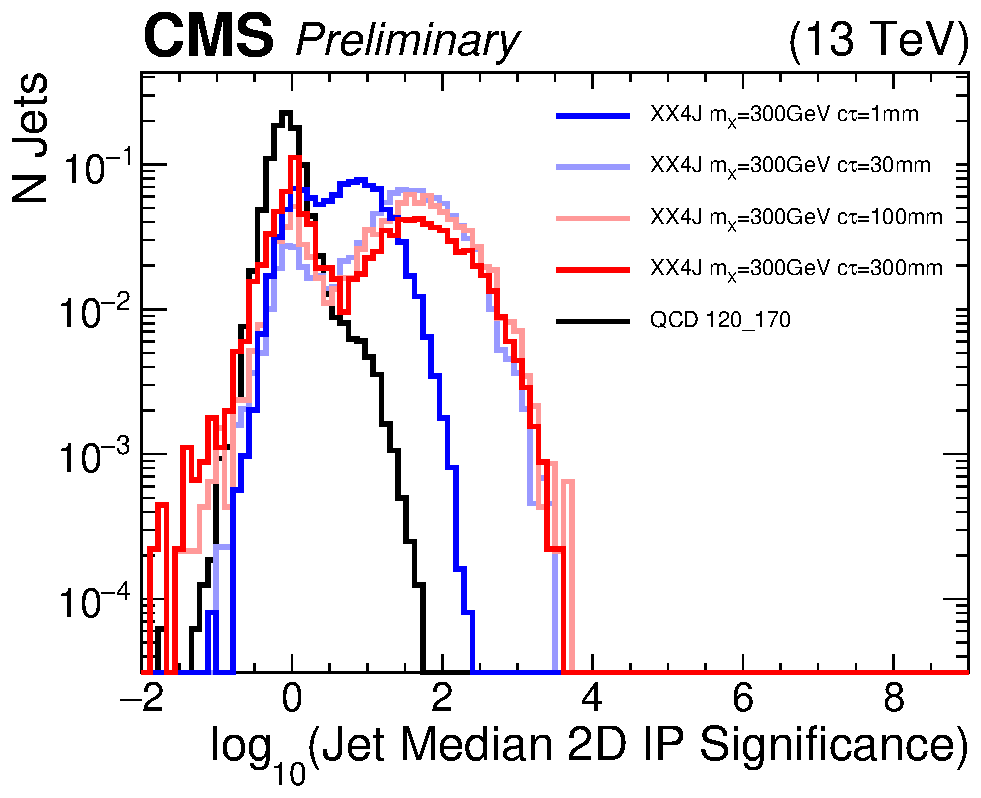
\includegraphics[width=.45\textwidth]{figures/an_jetid/VTX_MATCH_IP/XX4J_log_jetMedianIPSig2D}
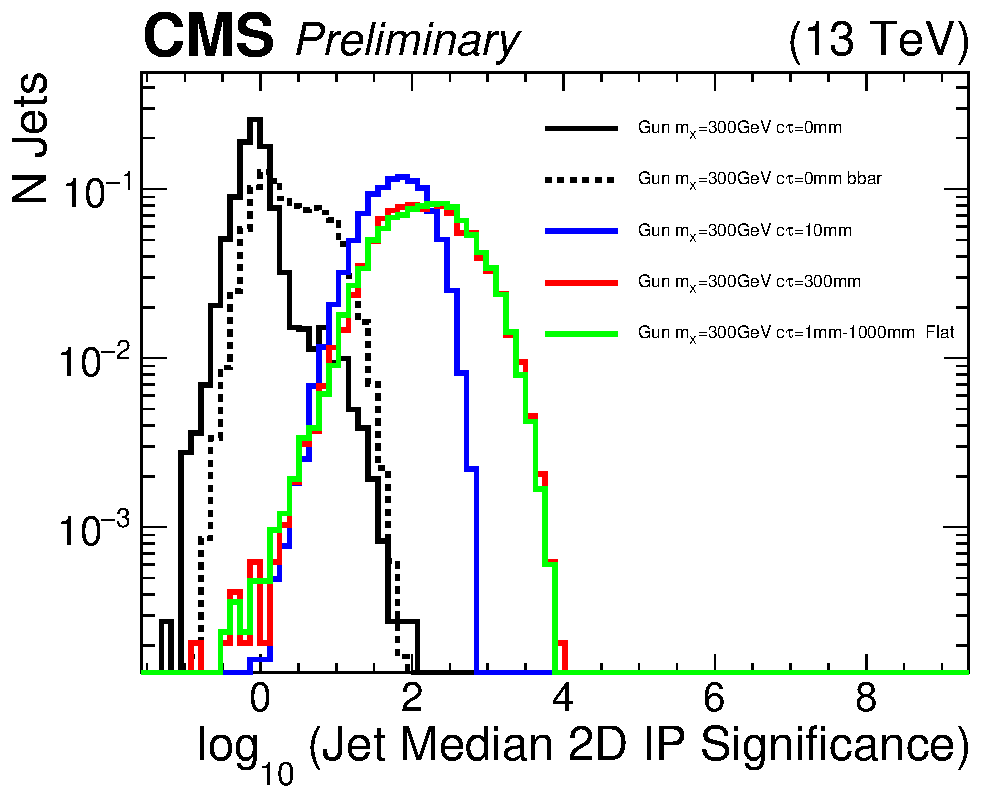
\includegraphics[width=.45\textwidth]{figures/an_jetid/VTX_MATCH_IP/GUN_log_jetMedianIPSig2D}
\end{center}
\caption{A comparison between using mean or median IP significance for the GUN and XX4J signal samples.}
\label{fig:ipsig_mean_median}
\end{figure}
Impact parameters are reconstructed with limited requirements on the tracks. No maximum longitudinal or transverse impact parameter
is enforced. No requirement on the number of hits, pixel tracks, or track quality is is required at this step. The tracks are required to have  $p_{\textrm{t}}>$ 1 GeV to remove tracks which would not reach the calorimeter face. 
%% \begin{verbatim}
%% displacedLifetimeTagInfos = cms.EDProducer( "TrackIPProducer",
%%     maximumTransverseImpactParameter = cms.double( 999999.0 ),
%%     minimumNumberOfHits = cms.int32( 0 ), 
%%     minimumTransverseMomentum = cms.double( 1.0 ),
%%     primaryVertex = cms.InputTag( 'offlinePrimaryVerticesWithBS'),
%%     maximumLongitudinalImpactParameter = cms.double( 999999.0 ), 
%%     computeGhostTrack = cms.bool( False ),
%%     ghostTrackPriorDeltaR = cms.double( 0.03 ),
%%     jetTracks = cms.InputTag( "displacedAk4JetTracksAssociatorAtVertex" ), 
%%     jetDirectionUsingGhostTrack = cms.bool( False ),
%%     minimumNumberOfPixelHits = cms.int32( 0 ), 
%%     jetDirectionUsingTracks = cms.bool( False ),
%%     computeProbabilities = cms.bool( False ),
%%     useTrackQuality = cms.bool( False ),
%%     maximumChiSquared = cms.double( 20.0 )
%% )
%% \end{verbatim}

Variables leveraging the impact parameter information  are derived from the distribution of impact parameter significances. 
Figure \ref{fig:ipsig_mean_median} demonstrates the improved  separation of median IP significance relative
 to the mean (Figure \ref{fig:ipsig_mean_median}). 
As background QCD jets contain real displaced tracks 
(Table \ref{tab:mesons}, \ref{tab:baryons}), the mean calculation is sensitive
 to outlier tracks with large IP significance. For signal-like displaced jets, 
all tracks have large impact parameter preserving a high median value. 
\begin{figure}
\begin{center}
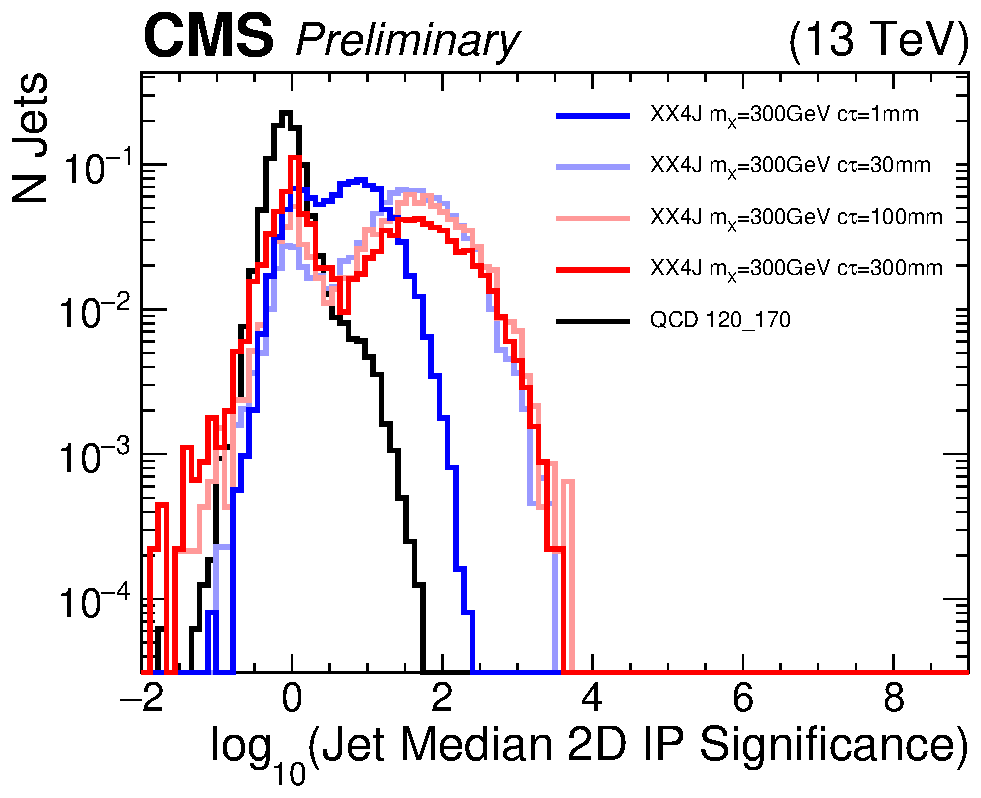
\includegraphics[width=.45\textwidth]{figures/an_jetid/VTX_MATCH_IP/XX4J_log_jetMedianIPSig2D}
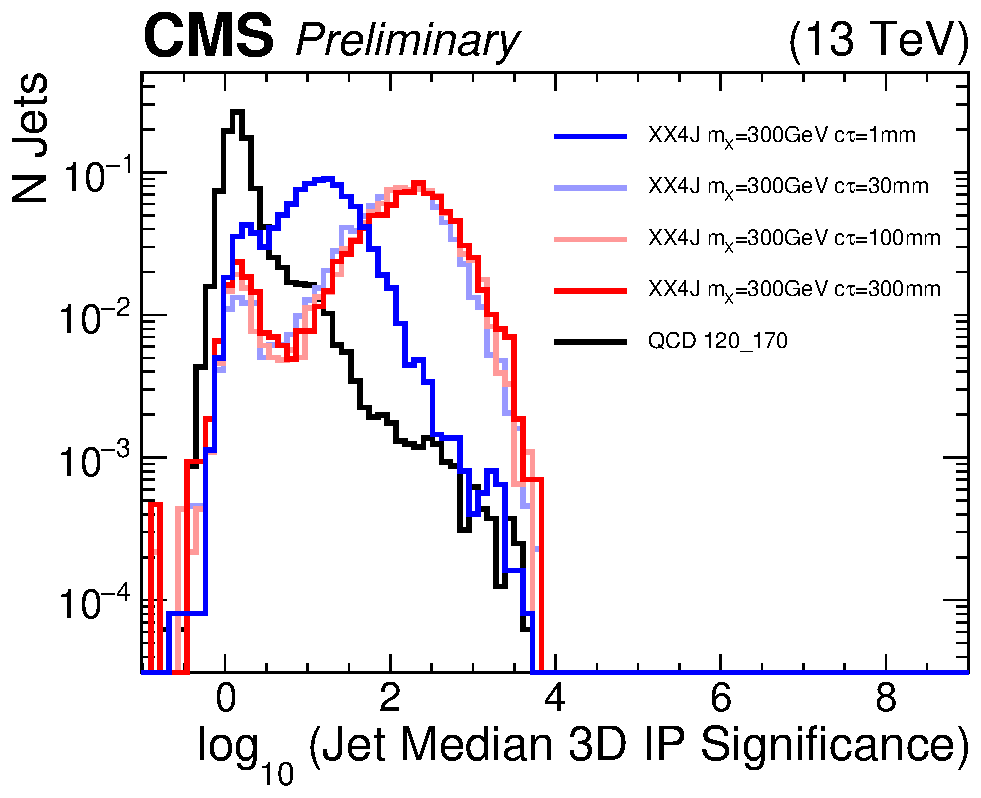
\includegraphics[width=.45\textwidth]{figures/an_jetid/VTX_MATCH_IP/XX4J_log_jetMedianIPSig3D}
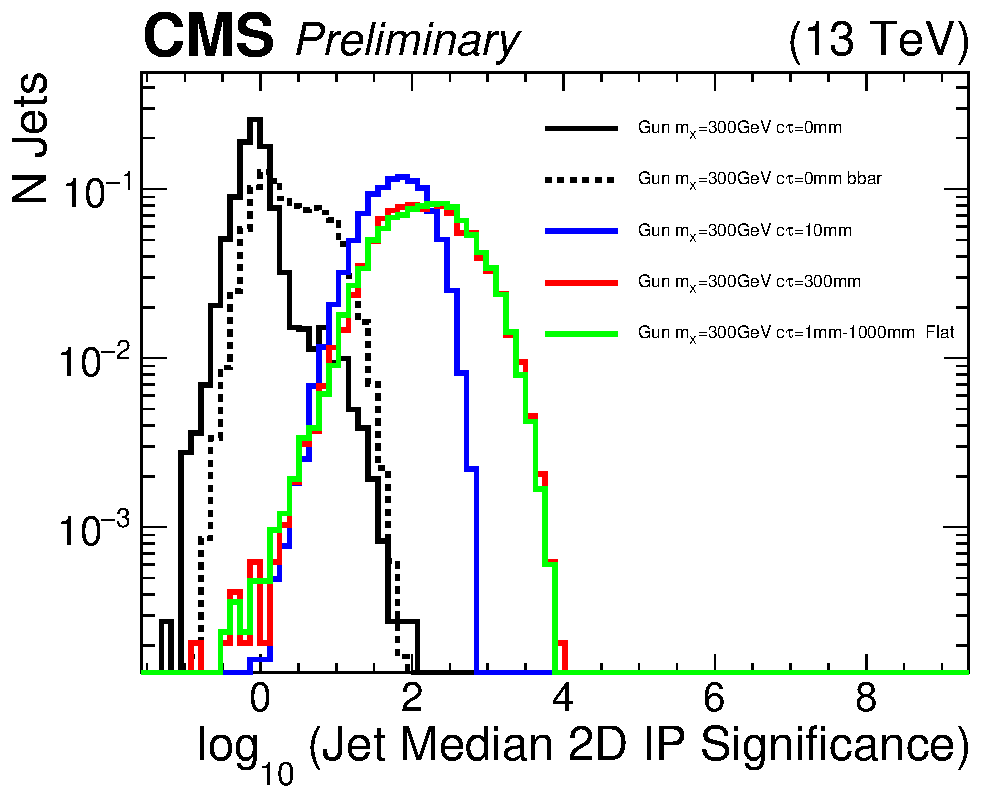
\includegraphics[width=.45\textwidth]{figures/an_jetid/VTX_MATCH_IP/GUN_log_jetMedianIPSig2D}
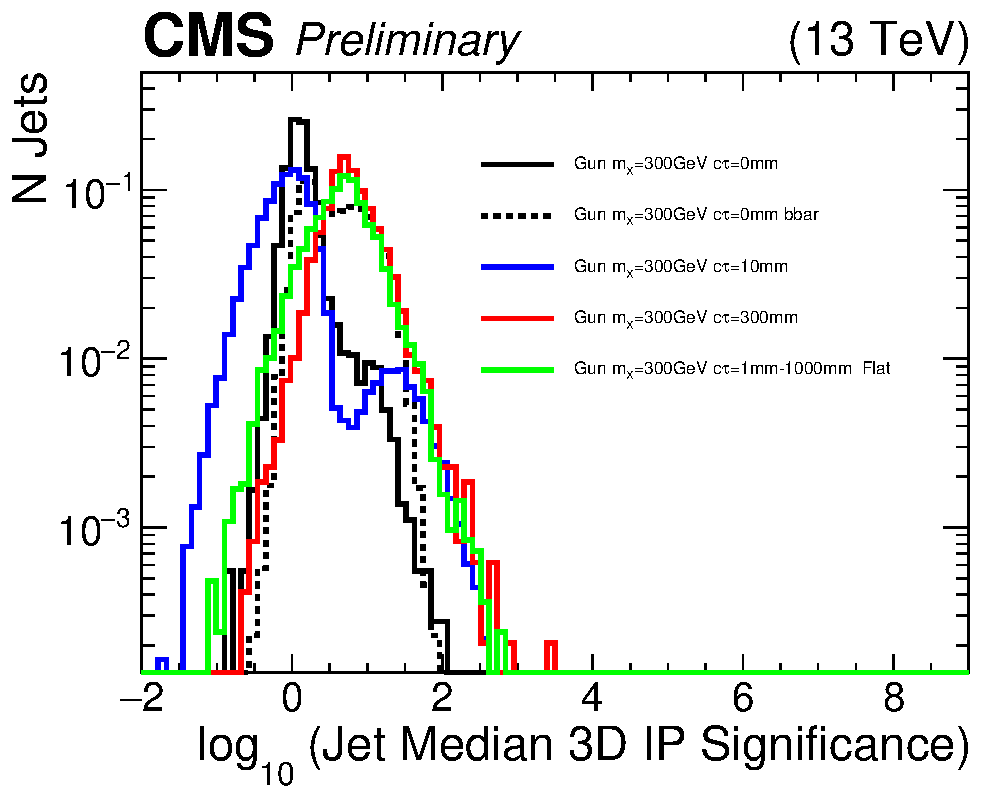
\includegraphics[width=.45\textwidth]{figures/an_jetid/VTX_MATCH_IP/GUN_log_jetMedianIPSig3D}
\end{center}
\caption{A comparison between the median IP significance in 2D vs 3D for the GUN and  XX4J signal samples}
\label{fig:ipsig_2d_3d}
\end{figure}

The tracks from displaced jets should not have significant contribution from tracks included in a primary vertex fit.
For long lifetimes this reduces the reliability of selecting the correct
primary vertex for the calculation of 3D impact parameters. Instead, the analysis opts to use exclusively transverse quantities that negligibly depend on the primary
 vertex selection when a beam-spot constraint is applied.  
Figure \ref{fig:ipsig_2d_3d} shows the comparison between the 2D and 3D
impact parameters. 3D distributions exhibit long tails where the wrong 
primary vertex was chosen. 

The choice is made to use report the value of impact parameter related variables
 on log scale. As impact parameter significance varies over many orders of 
magnitude (Figure \ref{fig:xx4j_iptrack}), the variable transformation 
reveals structure not visible on linear scales. On log scale, two populations 
of tracks are clearly visible.

\begin{figure}
\begin{center}
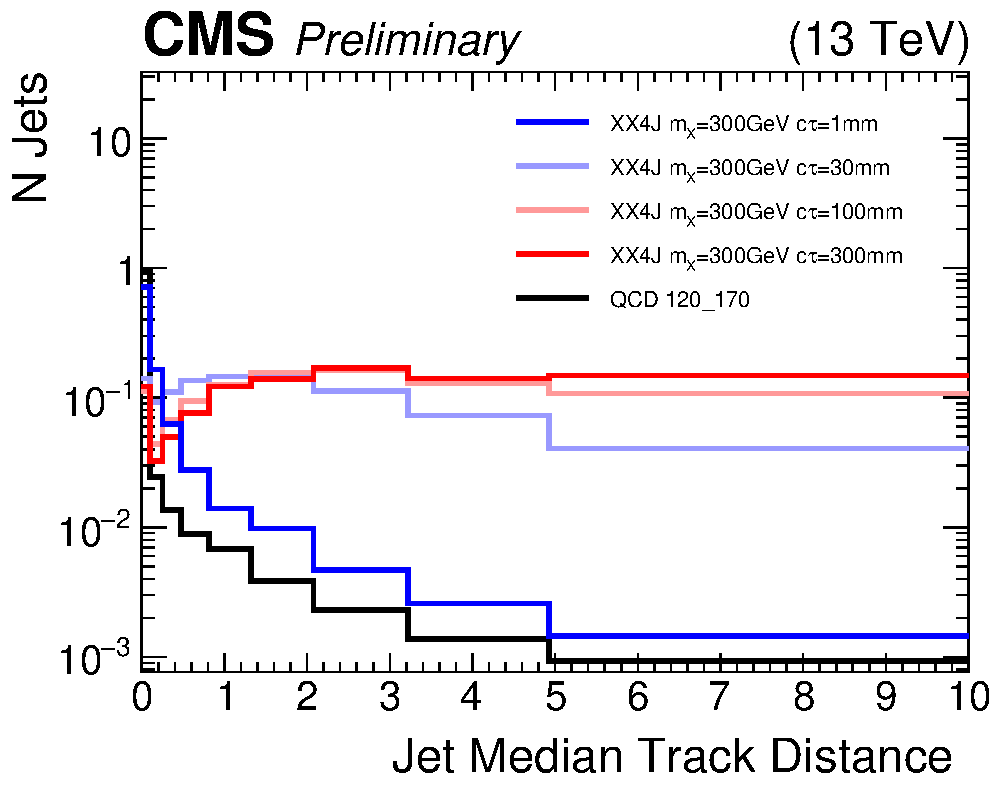
\includegraphics[width=.45\textwidth]{figures/an_jetid/VTX_MATCH_IP/XX4J_jetMedianDistance}
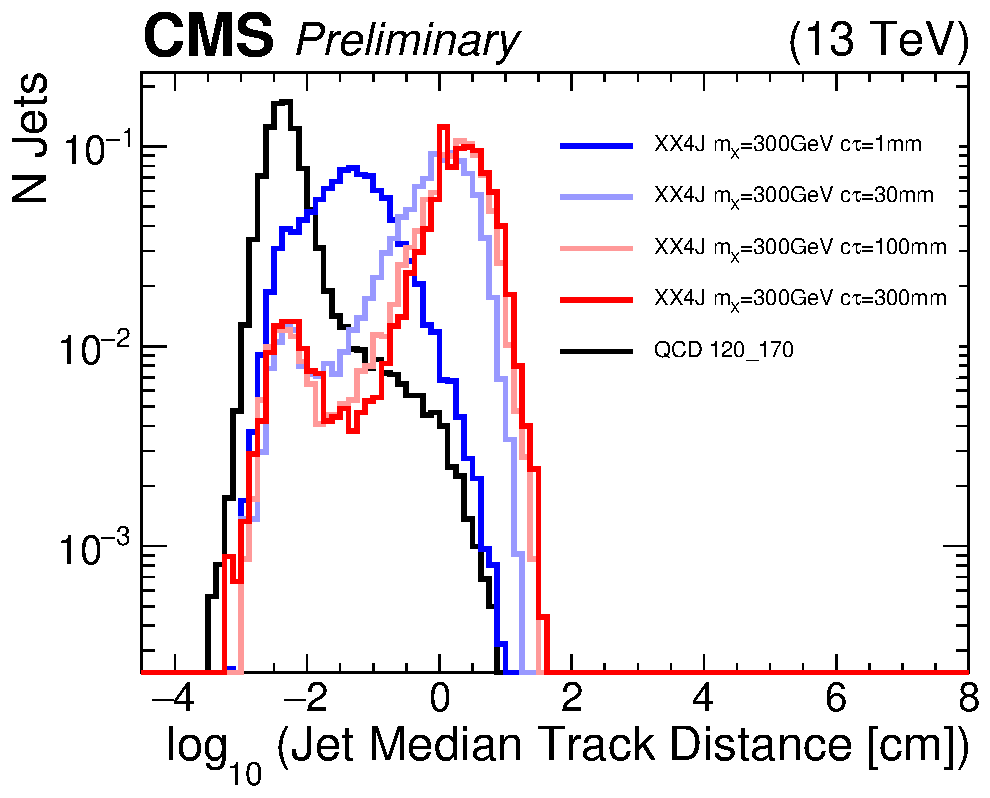
\includegraphics[width=.45\textwidth]{figures/an_jetid/VTX_MATCH_IP/XX4J_log_jetMedianTrackDist}
\end{center}
\caption{For each track in a jet the minimum distance between the track and the jet axis is computed. From this distribution
the median is computed for each jet.}
\label{fig:jetDistance}
\end{figure}

\begin{figure}
\begin{center}
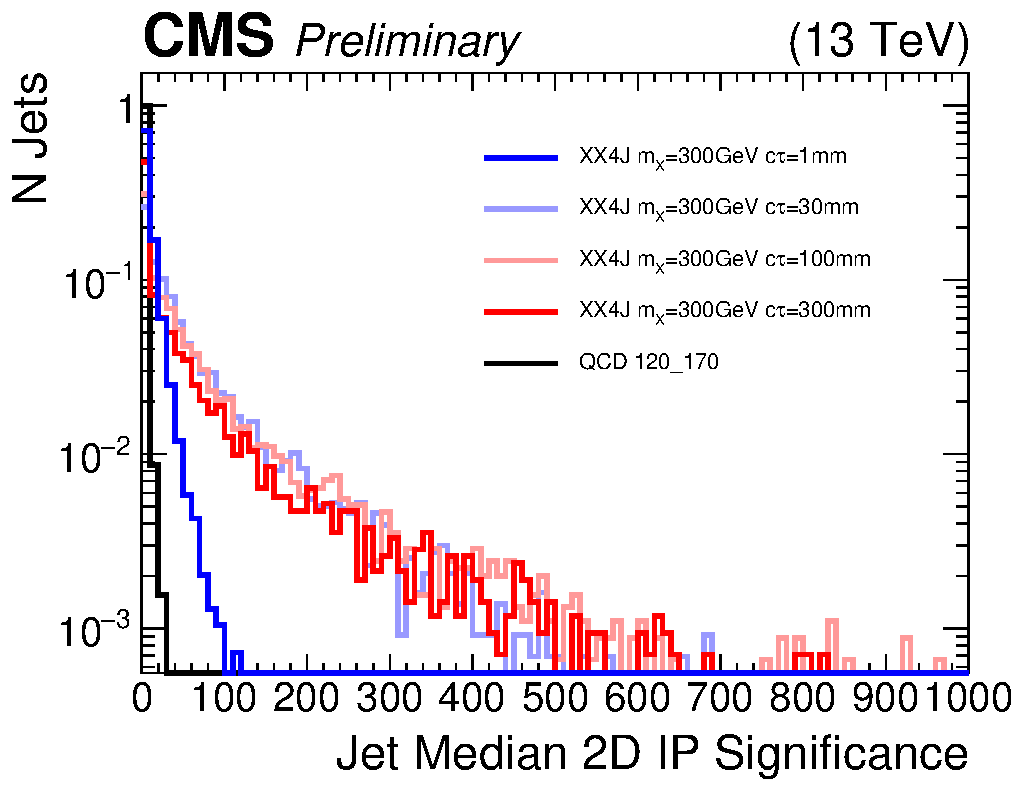
\includegraphics[width=.45\textwidth]{figures/an_jetid/VTX_MATCH_IP/XX4J_jetMedianIPSig2D}
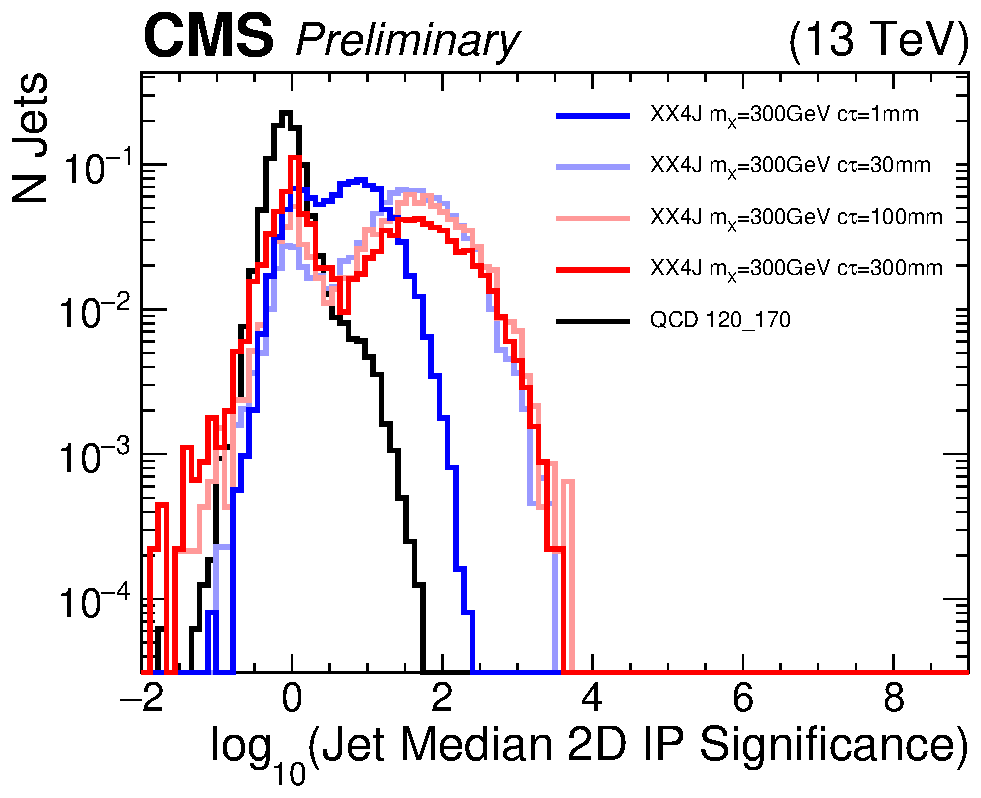
\includegraphics[width=.45\textwidth]{figures/an_jetid/VTX_MATCH_IP/XX4J_log_jetMedianIPSig2D}
\end{center}
\caption{A comparison between log and linear scale variables. The log scale case shows the distinct population
of significances related to pileup in the XX4J sample.}
\label{fig:xx4j_iptrack}
\end{figure}

\begin{figure}
\begin{center}
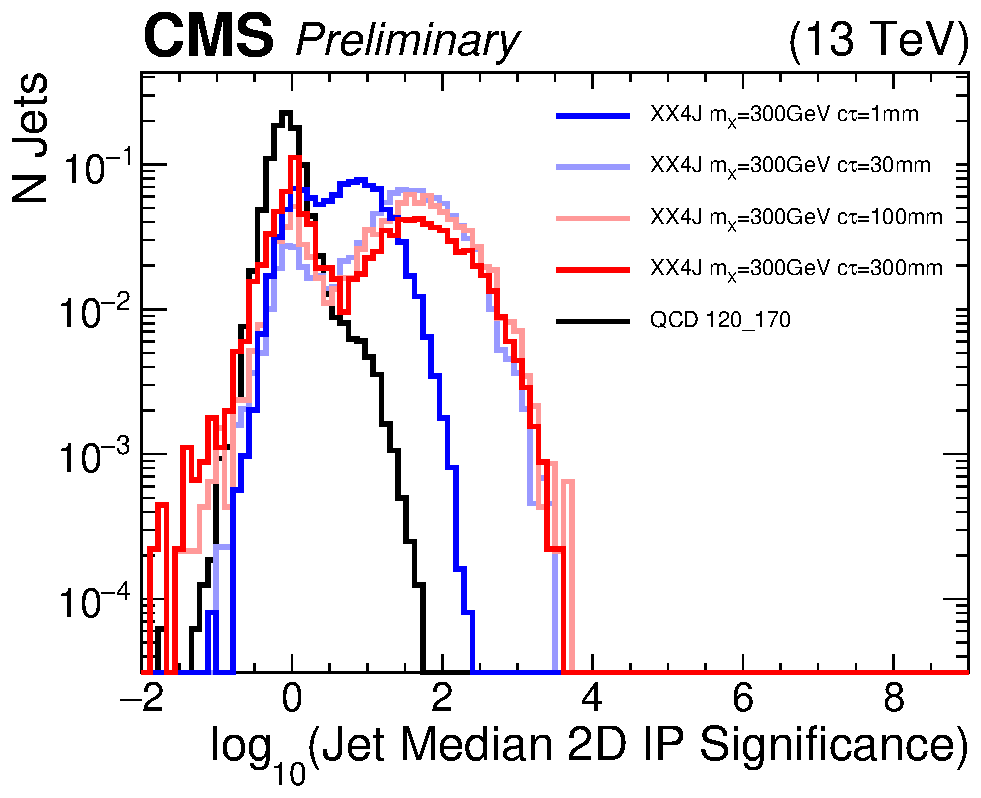
\includegraphics[width=.45\textwidth]{figures/an_jetid/VTX_MATCH_IP/XX4J_log_jetMedianIPSig2D}
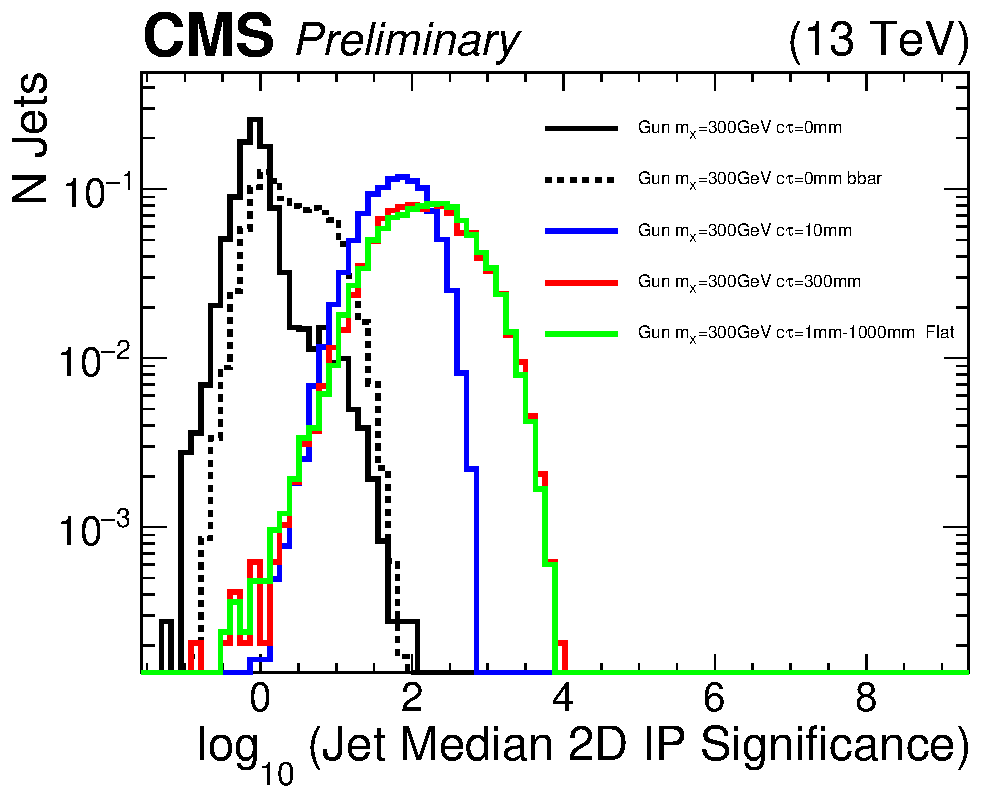
\includegraphics[width=.45\textwidth]{figures/an_jetid/VTX_MATCH_IP/GUN_log_jetMedianIPSig2D}
\end{center}
\caption{A comparison of the jet median 2D IP significance between the GUN and XX4J samples}
\label{fig:gun_ipsig}
\end{figure}

\begin{figure}
\begin{center}
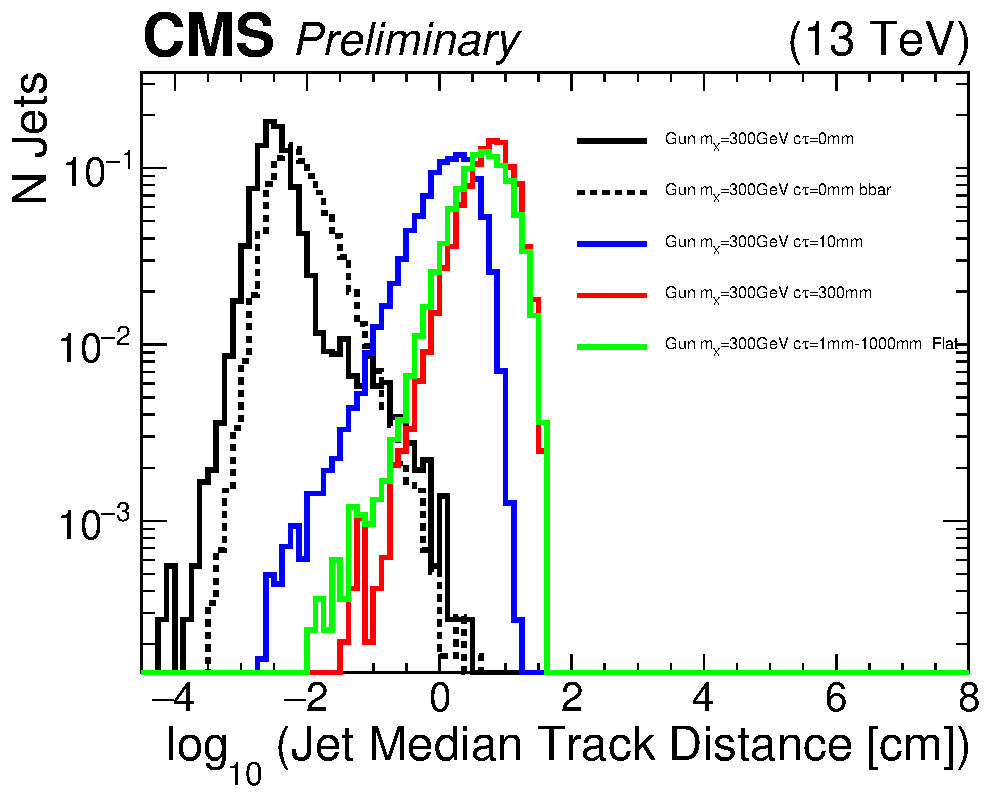
\includegraphics[width=.45\textwidth]{figures/an_jetid/VTX_MATCH_IP/GUN_log_jetMedianTrackDist}
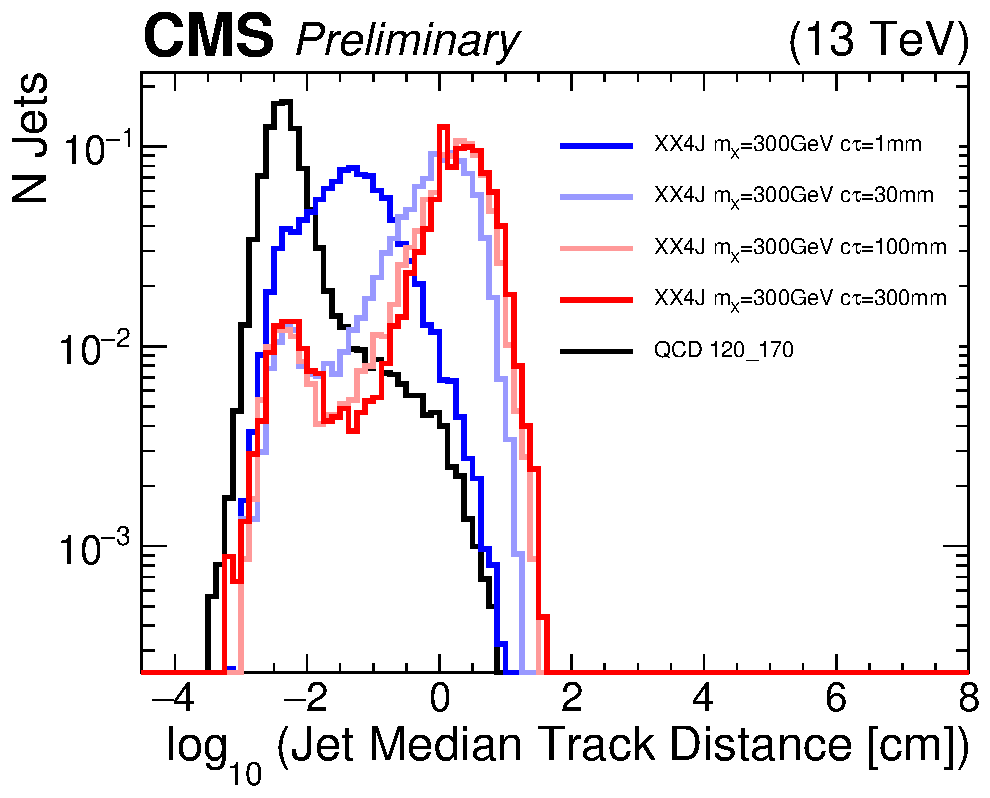
\includegraphics[width=.45\textwidth]{figures/an_jetid/VTX_MATCH_IP/XX4J_log_jetMedianTrackDist}
\end{center}
\caption{The closest distance between the jet axis and track for the GUN and XX4J samples}
\label{fig:jetDist}
\end{figure}

\begin{figure}
\begin{center}
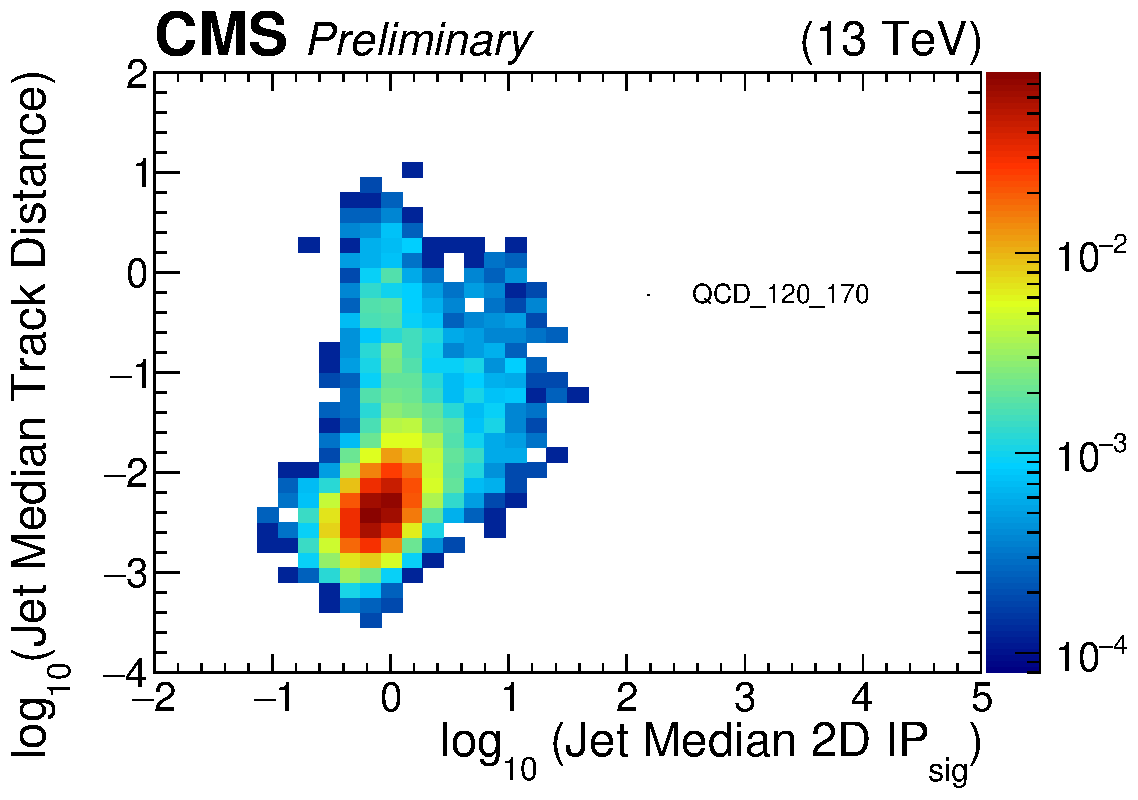
\includegraphics[width=.45\textwidth]{figures/an_jetid/VTX_MATCH_IP/QCD_2D_ipsig_jetDist}
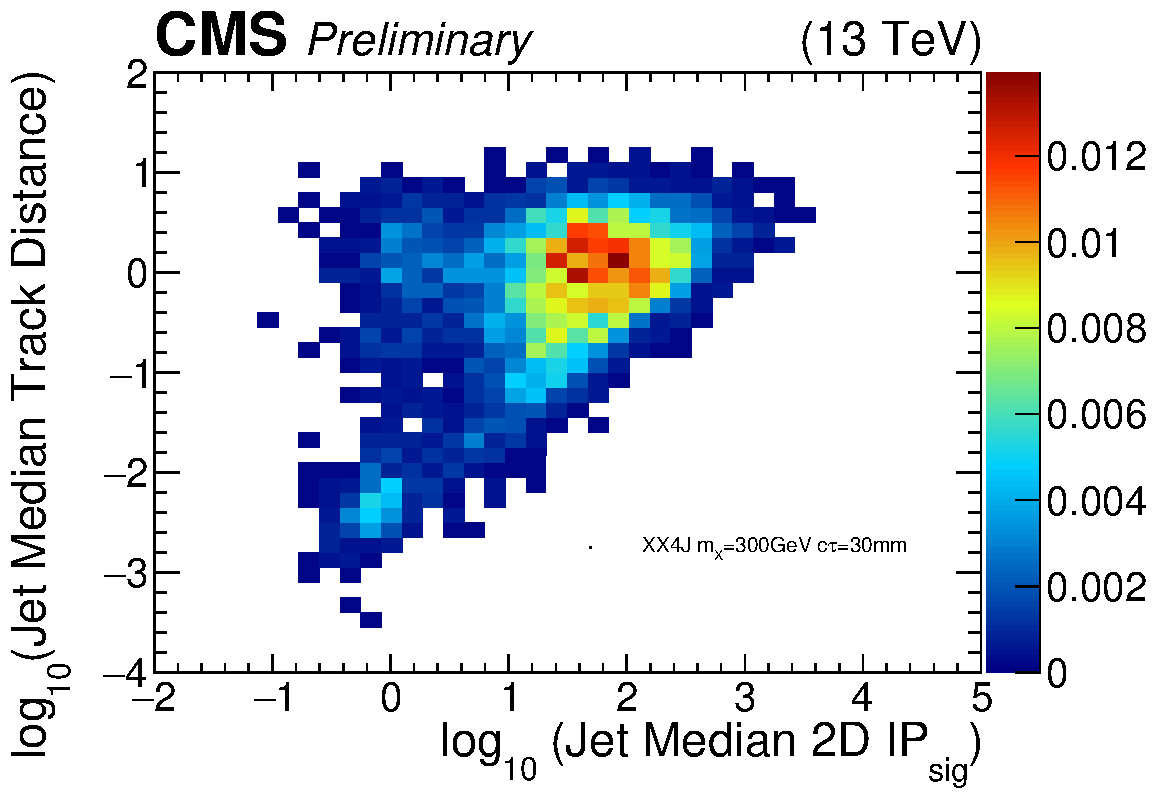
\includegraphics[width=.45\textwidth]{figures/an_jetid/VTX_MATCH_IP/XX4J_2D_ipsig_jetDist}
\end{center}
\caption{Correlations between the IP significance and the jet distance variables}
\label{fig:jetDist_ipsig}
\end{figure}

\subsubsection{Jet Primary Vertex Fraction ($\alpha$ and $\beta$)}

\begin{figure}
\begin{center}
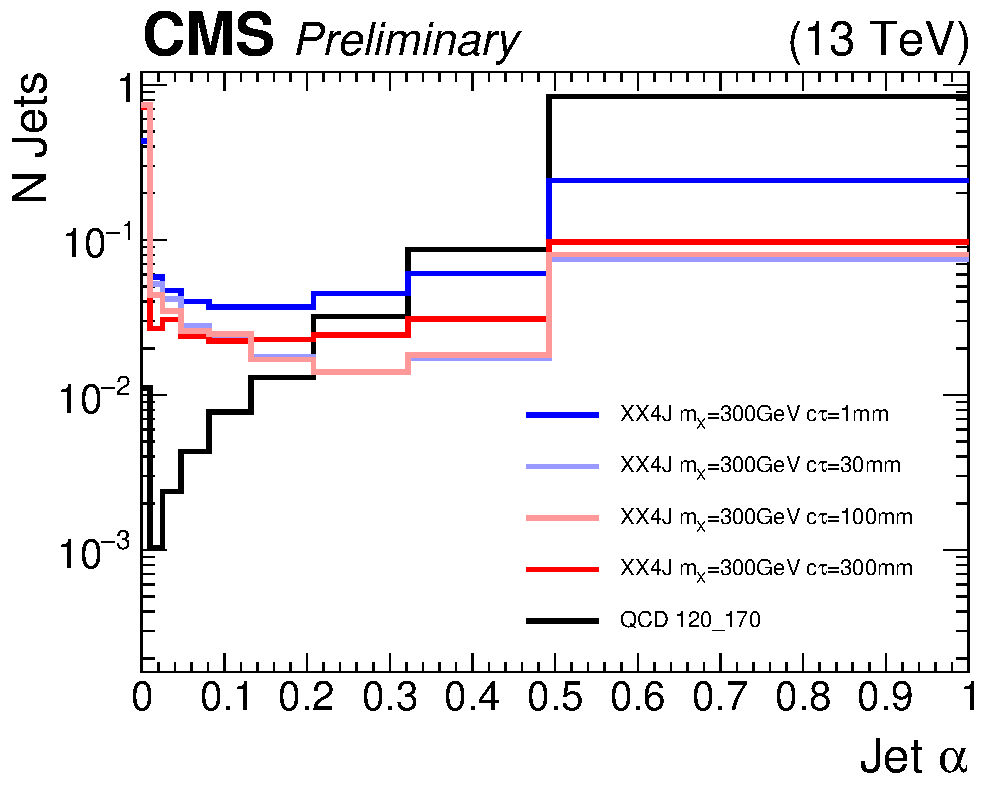
\includegraphics[width=.45\textwidth]{figures/an_jetid/VTX_MATCH_IP/XX4J_alpha}
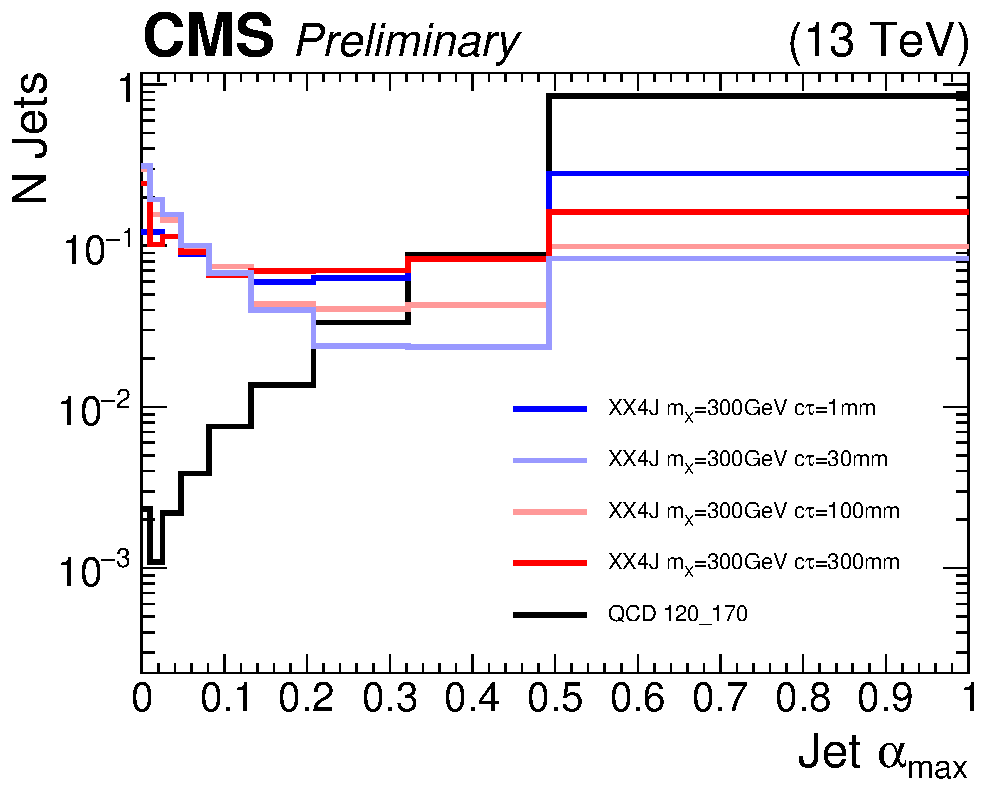
\includegraphics[width=.45\textwidth]{figures/an_jetid/VTX_MATCH_IP/XX4J_alphaMax}
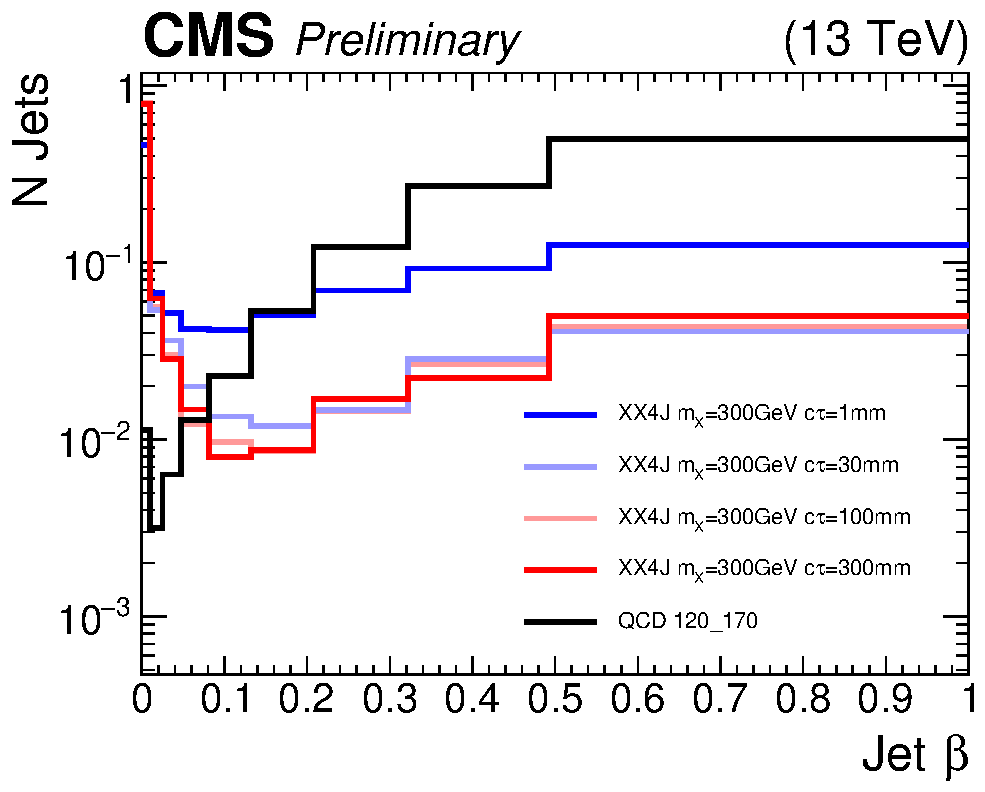
\includegraphics[width=.45\textwidth]{figures/an_jetid/VTX_MATCH_IP/XX4J_beta}
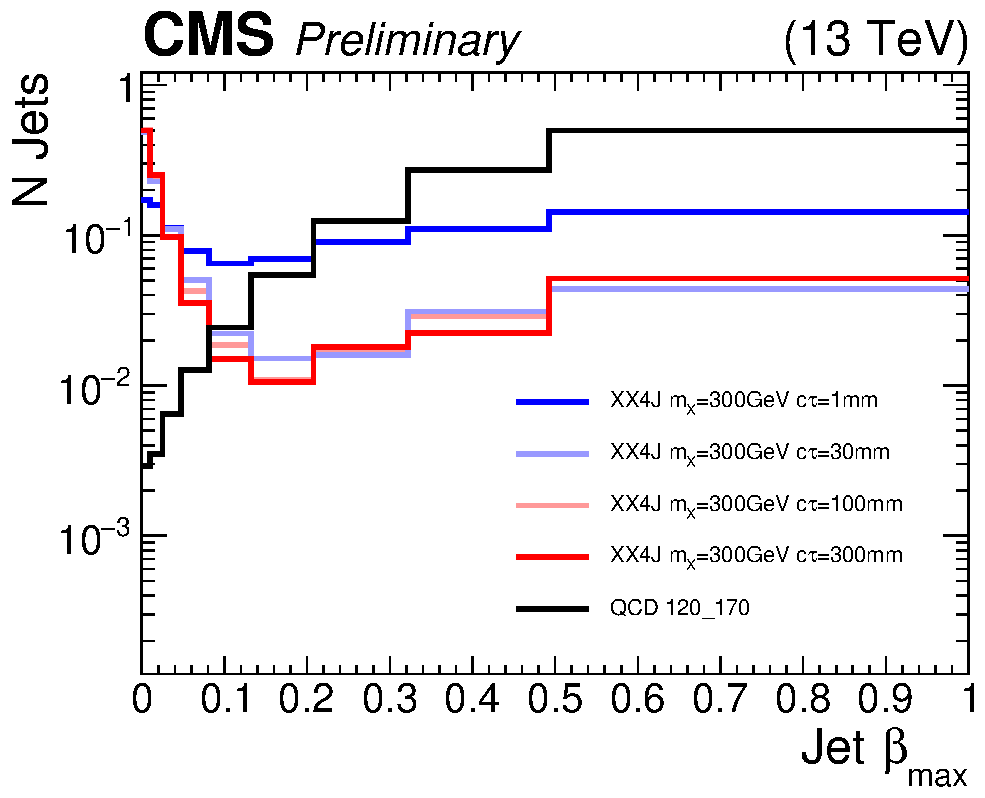
\includegraphics[width=.45\textwidth]{figures/an_jetid/VTX_MATCH_IP/XX4J_betaMax}
\end{center}
\caption{$\alpha, \alpha_{\textrm{max}}, \beta, \beta_{\textrm{max}}$ when varying the lifetime of the decaying $X^0$}
\label{fig:xx4j_alpha_beta}
\end{figure}

\begin{figure}
\begin{center}
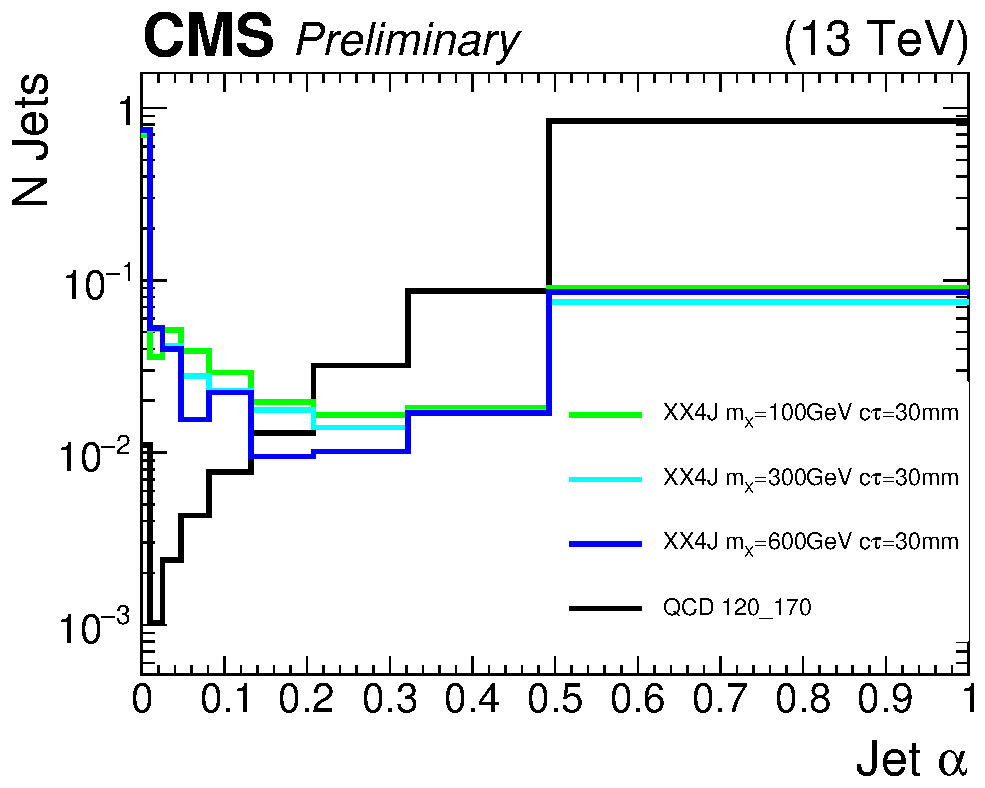
\includegraphics[width=.45\textwidth]{figures/an_jetid/VTX_MATCH_IP/XX4J_MASS_alpha}
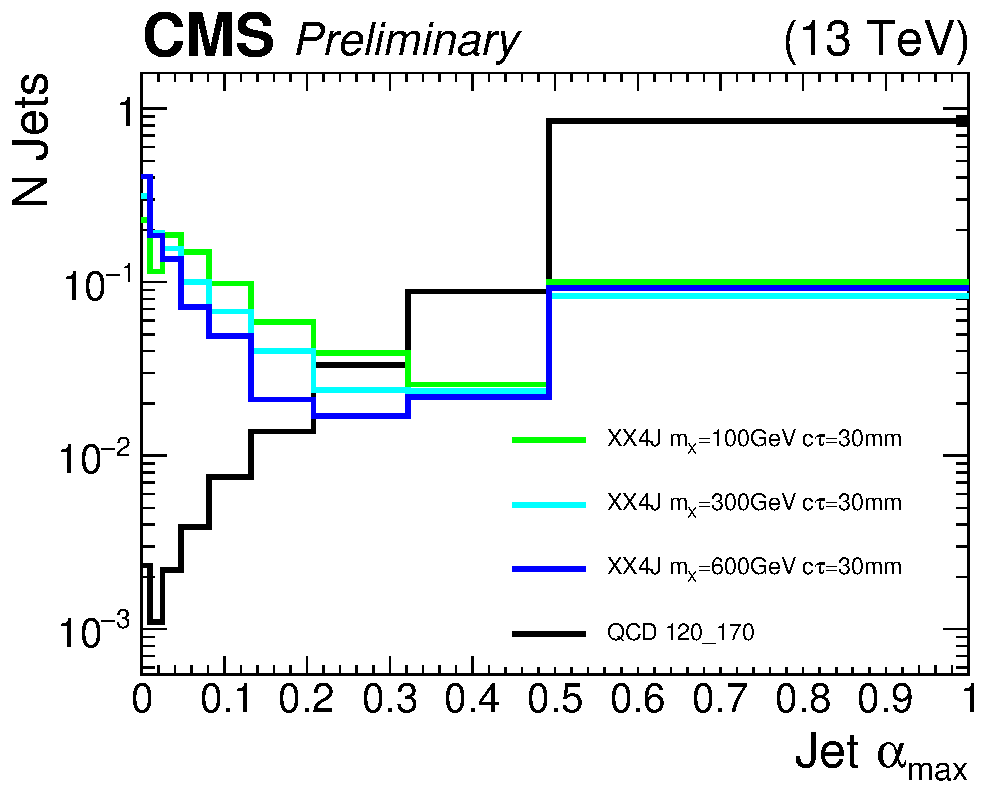
\includegraphics[width=.45\textwidth]{figures/an_jetid/VTX_MATCH_IP/XX4J_MASS_alphaMax}
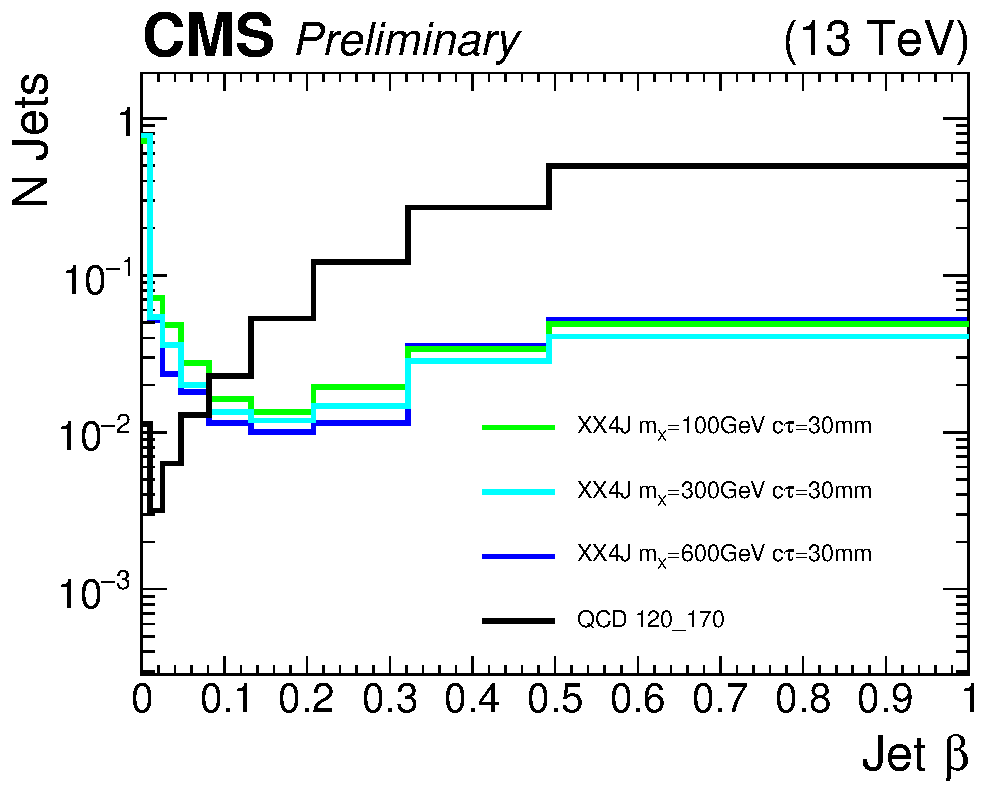
\includegraphics[width=.45\textwidth]{figures/an_jetid/VTX_MATCH_IP/XX4J_MASS_beta}
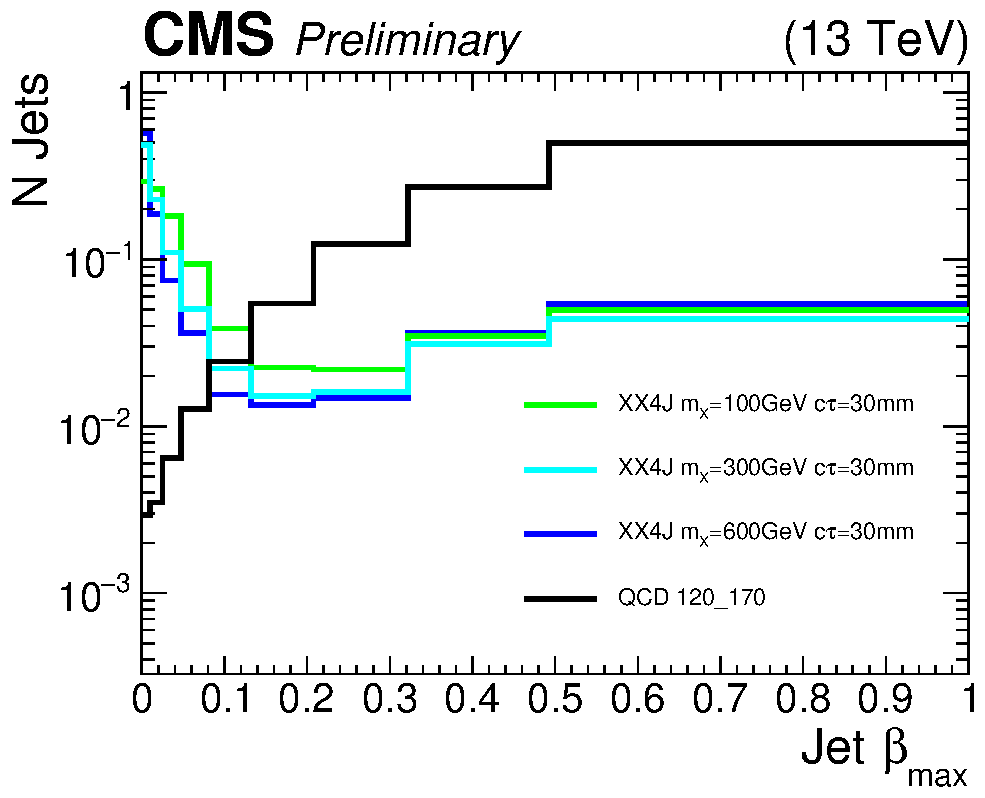
\includegraphics[width=.45\textwidth]{figures/an_jetid/VTX_MATCH_IP/XX4J_MASS_betaMax}
\end{center}
\caption{$\alpha, \alpha_{\textrm{max}}, \beta, \beta_{\textrm{max}}$ when varying the mass of the decaying $X^0$}
\label{fig:xx4j_mass_alpha_beta}
\end{figure}
Decays that occur displaced from the primary vertex are unlikely to contain tracks 
included in the primary vertex fit when a beam spot constraint is included.
On the other hand, QCD jets expect the majority of their tracks to be from either the true primary vertex or a pile up vertex.
For a given jet $\alpha(PV)$ is calculated as the sum is taken over tracks matching in $\Delta R< 0.4$ between two
collections of tracks: the tracks in the specified primary vertex and tracks from the global track collection. 
The sum is restricted to tracks with $p_{\textrm{t}} > 1.0$ GeV. 
\begin{equation}
\alpha_{\textrm{jet}}(\textrm{PV}) = \frac{\sum_{\textrm{tracks} \in \textrm{PV}} p_{\textrm{t}}^{\textrm{tracks}}}{\sum_{\textrm{tracks}} 
p_{\textrm{t}}^{\textrm{tracks}}}~,
\end{equation}
If the true PV is selected to calculate $\alpha$, PU jets will have have signal-like $\alpha=0$. 
To avoid this, we define $\alpha_{\textrm{max}}$ for each jet by individually selecting the primary vertex with
the largest contribution to the sum. As the GUN samples typically have no reconstructed primary vertices
 (except in the prompt case), these plots are not shown. 

A second jet variable $\beta(\textrm{PV})$ and $\beta_{\textrm{max}}$ are defined similarly:
%% \begin{equation}
%% \beta_{jet}(PV) = \frac{\sum_{i \in PV,tracks} p_{t}^i}{p_{t,jet}}
%% \end{equation}
\begin{equation}
\beta_{\textrm{jet}}(\textrm{PV}) = \frac{\sum_{\textrm{tracks} \in \textrm{PV}} p_{\textrm{t}}^{\textrm{tracks}}}{p_{\textrm{t}}^{\textrm{jet}}}~,
\end{equation}
A comparison of the four variables: $\alpha, \alpha_{\textrm{max}}, \beta, \beta_{\textrm{max}}$ is shown in 
Figure \ref{fig:xx4j_alpha_beta} by varying the lifetime of the sample. In Figure \ref{fig:xx4j_mass_alpha_beta} the same
comparison is made but varying the mass and leaving the lifetime fixed. 
\begin{figure}
\begin{center}
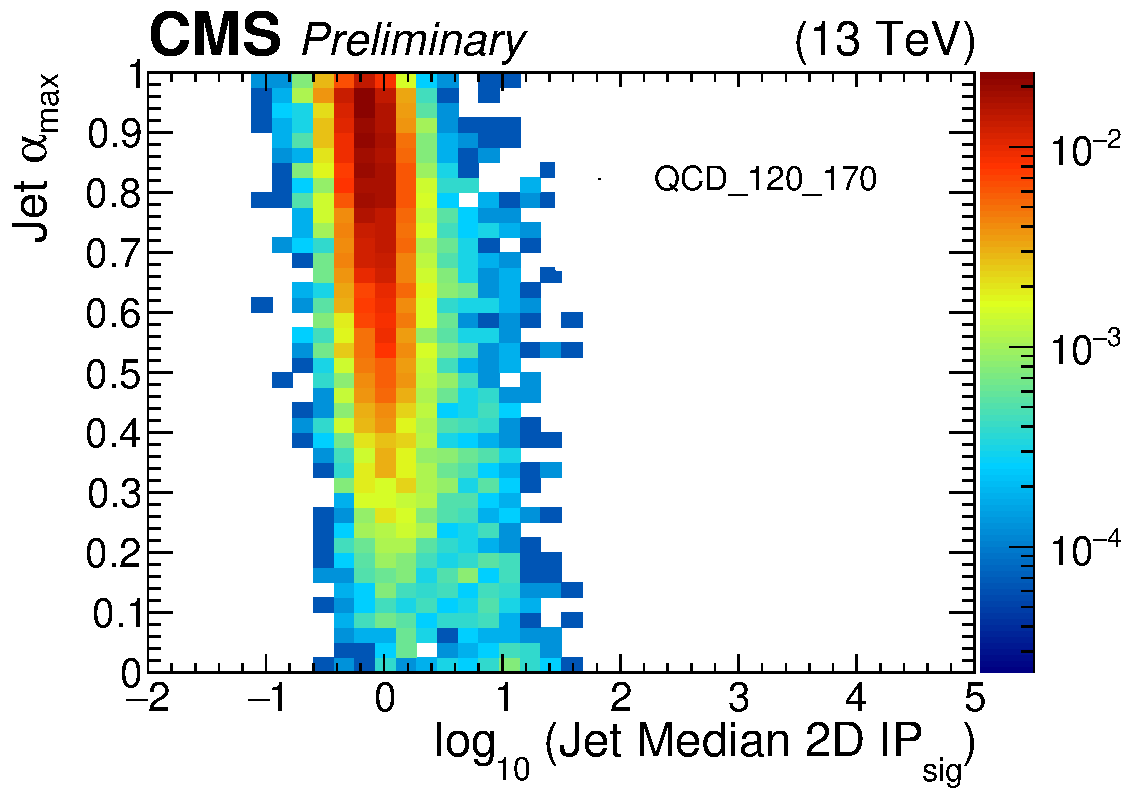
\includegraphics[width=.45\textwidth]{figures/an_jetid/VTX_MATCH_IP/QCD_2D_medianipsig_alpha}
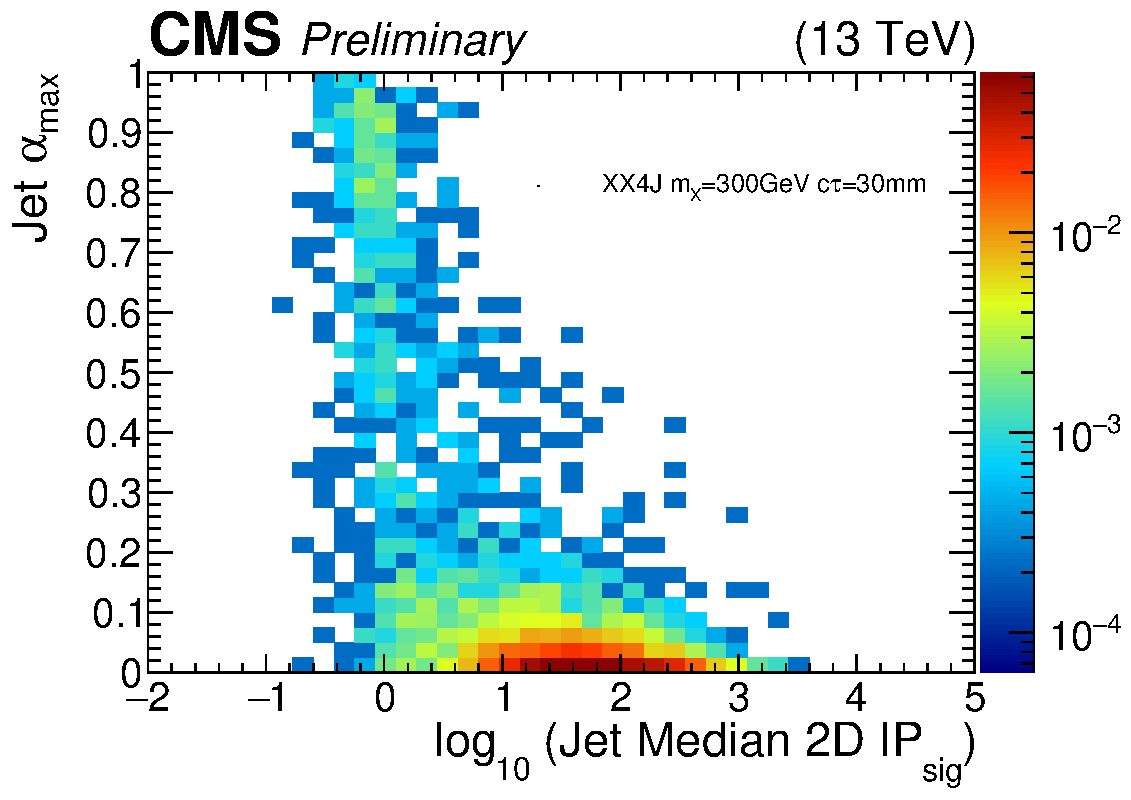
\includegraphics[width=.45\textwidth]{figures/an_jetid/VTX_MATCH_IP/XX4J_2D_medianipsig_alpha}
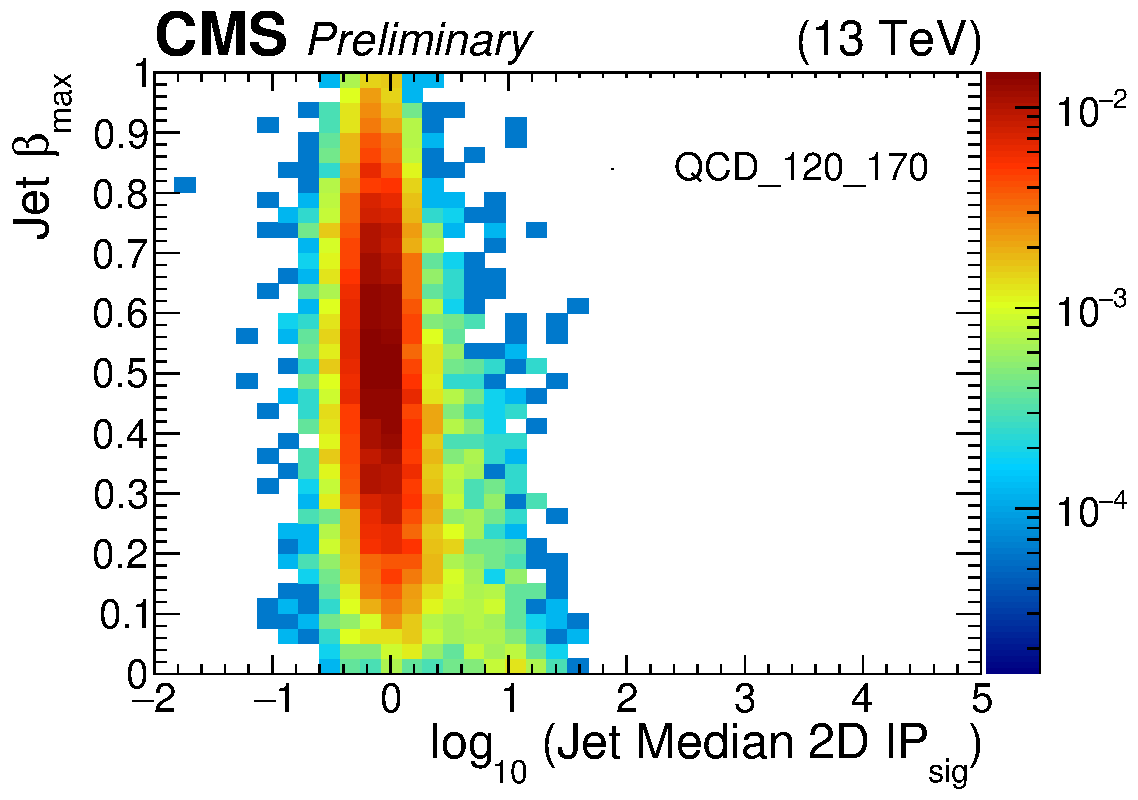
\includegraphics[width=.45\textwidth]{figures/an_jetid/VTX_MATCH_IP/QCD_2D_medianipsig_beta}
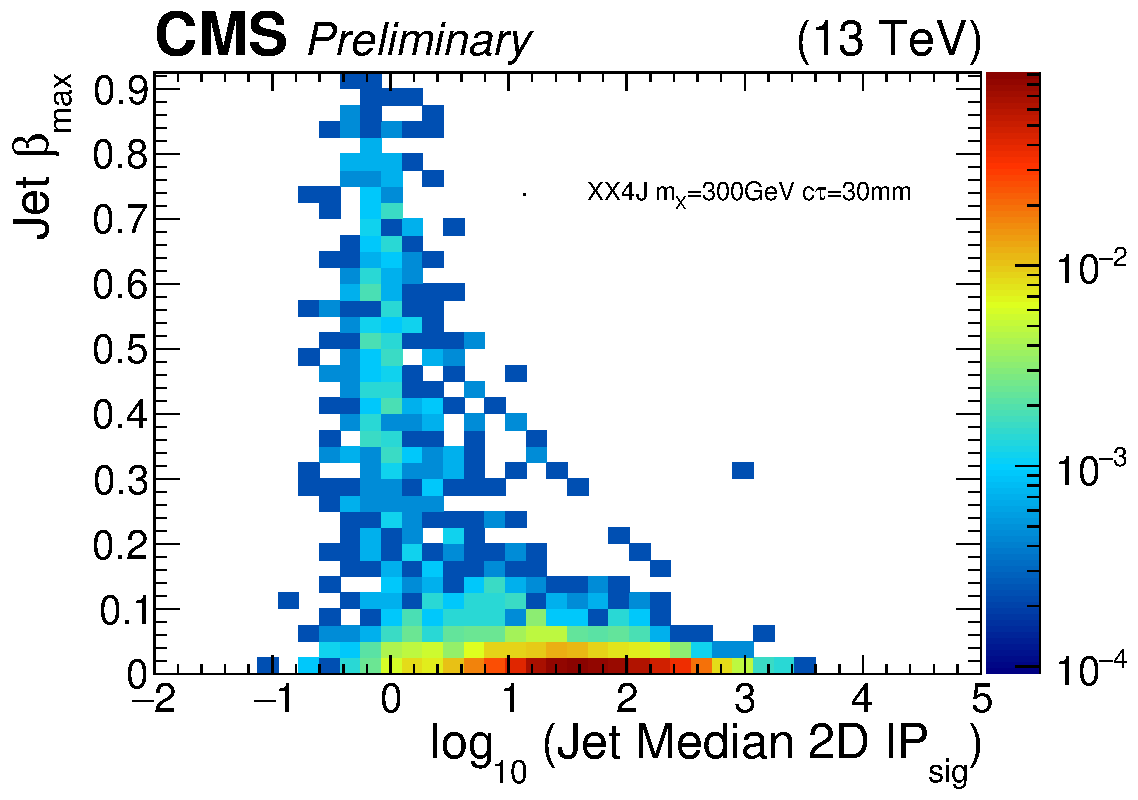
\includegraphics[width=.45\textwidth]{figures/an_jetid/VTX_MATCH_IP/XX4J_2D_medianipsig_beta}
\end{center}
\caption{(left) The correlation between $\alpha_{\textrm{max}}$ and $\beta_{\textrm{max}}$ and median 2D IP significance for QCD. (right) 
The same correlation plot for XX4J with $m_{X^0}=300$ GeV and $c\tau_0 = 30$ mm}
\label{fig:2d_alpha_beta_ipsig}
\end{figure}
Figure \ref{fig:2d_alpha_beta_ipsig} shows $\alpha_{\textrm{max}}$ has small correlation in background with the median 2D IP significance
and $\beta_{\textrm{max}}$ less so. This is because $\alpha_{\textrm{max}}$ is a function of the tracks matched to the jet, 
which are utilized in the median IP significance calculation. 
\subsection{Calo Jet Information}
\begin{figure}
\begin{center}
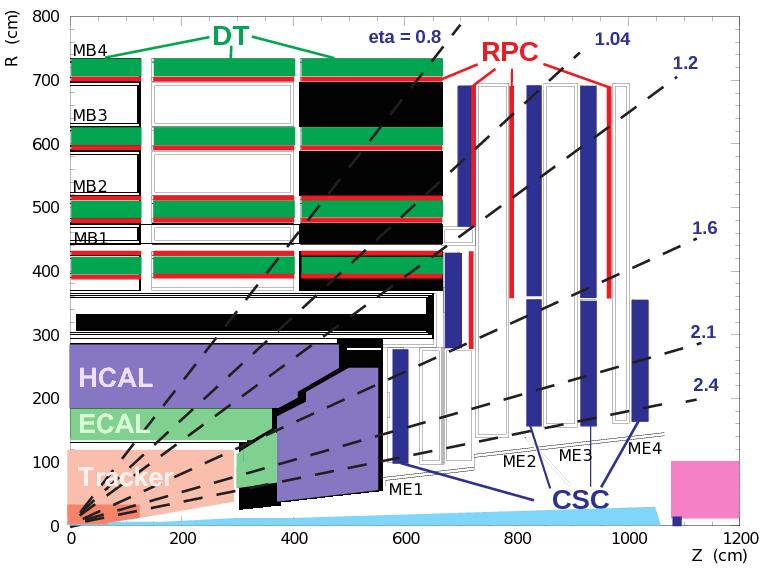
\includegraphics[width=.45\textwidth]{figures/an_jetid/DIAGRAMS/cms_slice}
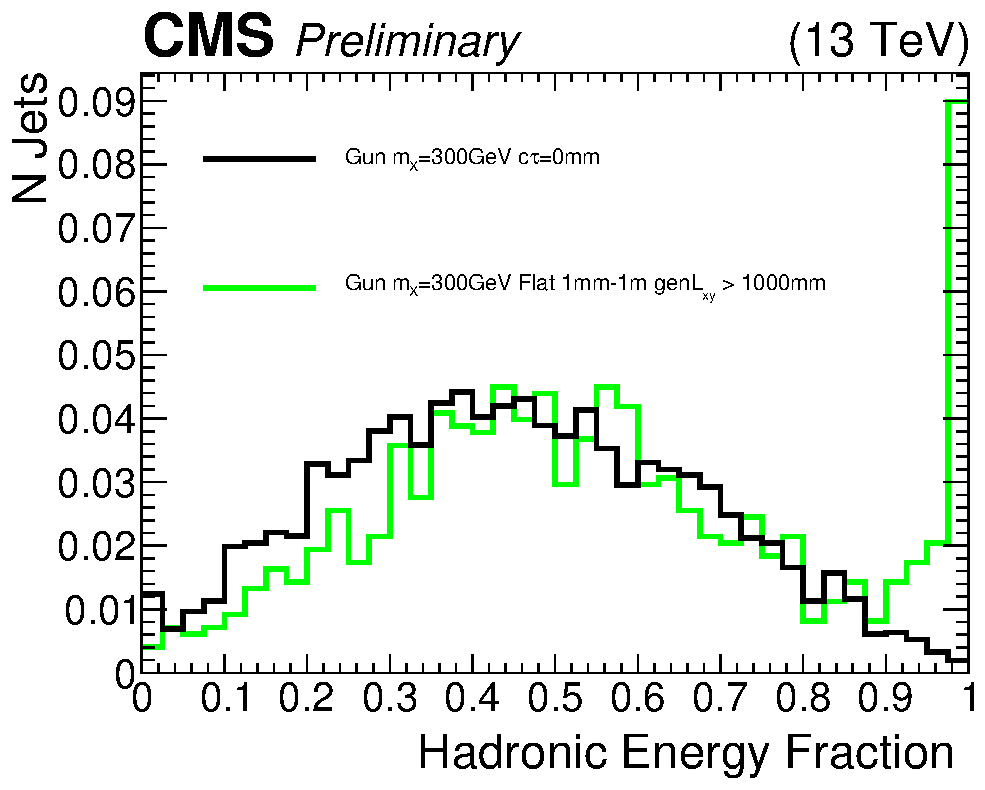
\includegraphics[width=.45\textwidth]{figures/an_jetid/VTX_MATCH_IP/GUN_hadronicFraction}
\end{center}
\caption{(left) A longitudinal slice of the CMS detector showing the transverse coverage of the tracking layers. (right) Hadronic fraction of jets in events with generator level requirement that the $X^{0}$ decay at a transverse distance $L_{xy} > 100$ cm}
\label{fig:hadronicFraction}
\end{figure}
In the case which there are no tracks to identify the decay as 
displaced, we can utilize the high hadronic energy fraction
of jets that occur from long-lived decays inside of the hadronic calorimeter. 
Figure \ref{fig:hadronicFraction} includes a generator level
cut on the transverse decay distance of $>1$ m to ensure that the decay occurs outside of the tracker.
